\documentclass[10pt,twocolumn,a4paper]{article}

% --- Essential Packages ---
\usepackage[utf8]{inputenc}
\usepackage[margin=0.72in, top=0.75in, bottom=0.75in, columnsep=18pt]{geometry}
\usepackage{amsmath,amssymb,amsfonts}
\usepackage{booktabs}
\usepackage{graphicx}
\usepackage{subcaption}
\usepackage{caption}
\usepackage{hyperref}
\usepackage{microtype}
\usepackage{tikz}
\usetikzlibrary{shapes.geometric, arrows.meta, positioning, calc}
\usepackage{xcolor}
\usepackage{enumitem}
\usepackage{titlesec}

% --- Hyperref Setup ---
\hypersetup{
    colorlinks=true,
    linkcolor=blue!70!black,
    citecolor=blue!70!black,
    urlcolor=blue!70!black
}

% --- Custom Formatting & Spacing ---
\setlength{\parindent}{1.2em}
\setlength{\parskip}{0.15em}
\titlespacing*{\section}{0pt}{1.2ex plus 0.3ex minus 0.1ex}{0.5ex plus 0.1ex}
\titlespacing*{\subsection}{0pt}{1.0ex plus 0.2ex minus 0.1ex}{0.4ex plus 0.1ex}
\titlespacing*{\subsubsection}{0pt}{0.8ex plus 0.2ex minus 0.1ex}{0.3ex plus 0.1ex}

% --- Document Title & Metadata ---
\title{\vspace{-1.2em}\textbf{\Large Dynamics and Processes on Complex Networks (DPCN)}\\\vspace{0.25em}
\textbf{\large Assignment 1: Opinion Network Formation \& Structural Analysis}\\\vspace{0.25em}
\normalsize Quantitative Modeling of Ideological Alignment, Thematic Communities, and Percolation Transitions}

\author{
    \textbf{Team Name: Lost in the Network} \\[0.3em]
    \normalsize
    \begin{tabular}{ccc}
        \textbf{Ampilli Sai Venkata Naga Bhargav} & \textbf{Chaitanya Thogata} & \textbf{Pasumarthy Deepak} \\
        (\textit{2023112014}) & (\textit{2023113018}) & (\textit{2023101109})
    \end{tabular}\\[0.25em]
}
% \date{\vspace{-0.5em}\small September 2026}

\begin{document}

\maketitle

% ==============================================================================
% SECTION 1: TEAM INFORMATION
% ==============================================================================
\section{Team Information}
\label{sec:team}

\begin{itemize}[noitemsep,topsep=1pt,leftmargin=1.2em]
    \item \textbf{Team Name:} \texttt{Lost in the Network}
    \item \textbf{Group Members and Roll Numbers:}
    \begin{enumerate}[noitemsep,topsep=1pt,leftmargin=1.2em]
        \item \textbf{Ampilli Sai Venkata Naga Bhargav} --- Roll Number: \texttt{2023112014}
        \item \textbf{Chaitanya Thogata} --- Roll Number: \texttt{2023113018}
        \item \textbf{Pasumarthy Deepak} --- Roll Number: \texttt{2023101109}
    \end{enumerate}
    \item \textbf{Course:} Dynamics and Processes on Complex Networks (DPCN)
\end{itemize}

% ==============================================================================
% SECTION 2: GITHUB LINK
% ==============================================================================
\section{GitHub Link to Code Repository}
\label{sec:github}

The complete source code, preprocessing modules, network construction algorithms, high-resolution figures, and reproducible execution pipelines are publicly hosted at:
\begin{center}
    \url{https://github.com/saiXbhargav/DPCN_assignment1}
\end{center}
The repository is organized modularly: pipeline execution is automated by \texttt{run\_pipeline.py}, core algorithms reside in \texttt{src/}, raw survey responses are provided in \texttt{Survey\_Results\_UC.csv}, and all verified outputs and publication figures are generated into \texttt{output/}.

% --- Pre-queue Figure 1 so it appears cleanly at the top of Page 2 ---
\begin{figure*}[t]
\centering
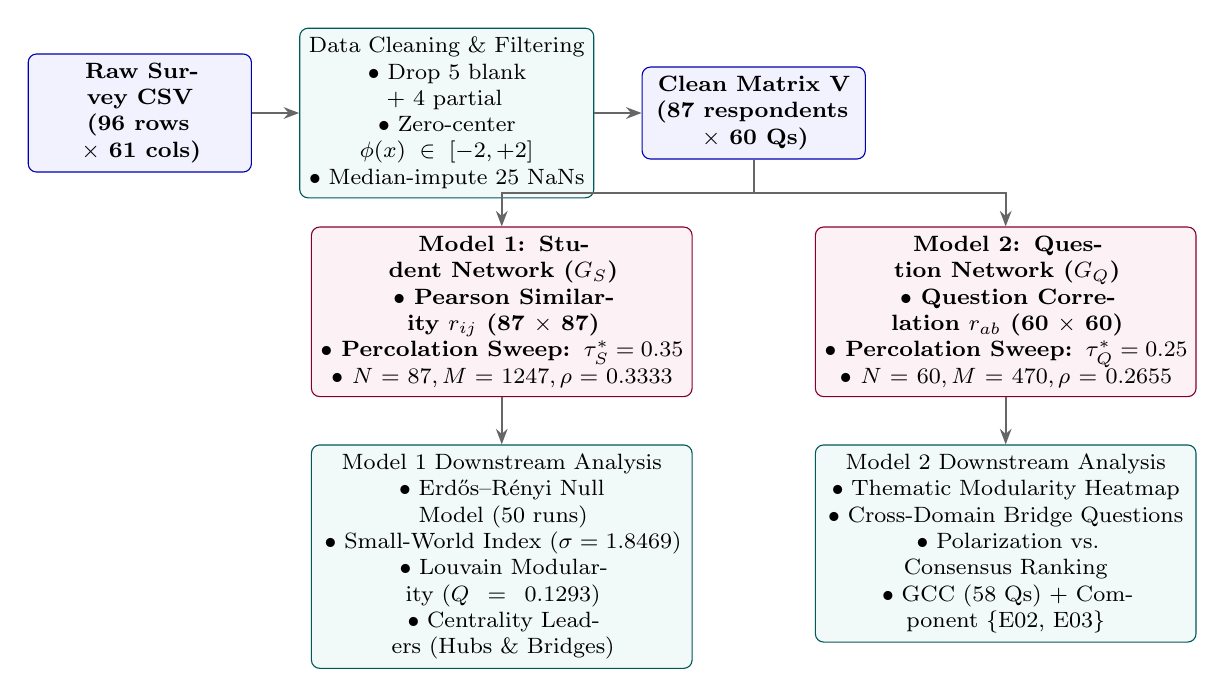
\begin{tikzpicture}[
    node distance=0.8cm and 0.8cm,
    box/.style={rectangle, draw=blue!70!black, fill=blue!5, rounded corners=3pt, text centered, minimum height=0.75cm, font=\footnotesize\bfseries},
    proc/.style={rectangle, draw=teal!70!black, fill=teal!5, rounded corners=3pt, text centered, minimum height=0.75cm, font=\footnotesize},
    model/.style={rectangle, draw=purple!70!black, fill=purple!5, rounded corners=3pt, text centered, minimum height=0.75cm, font=\footnotesize\bfseries},
    arrow/.style={-{Stealth[scale=0.85]}, thick, draw=gray!80!black}
]
    \node (raw) [box, text width=2.6cm] {Raw Survey CSV\\(96 rows $\times$ 61 cols)};
    \node (prep) [proc, right=0.6cm of raw, text width=3.5cm] {Data Cleaning \& Filtering\\$\bullet$ Drop 5 blank + 4 partial\\$\bullet$ Zero-center $\phi(x) \in [-2, +2]$\\$\bullet$ Median-impute 25 NaNs};
    \node (mat) [box, right=0.6cm of prep, text width=2.6cm] {Clean Matrix $\mathbf{V}$\\(87 respondents $\times$ 60 Qs)};
    
    \node (m1) [model, below=0.85cm of mat, xshift=-3.2cm, text width=4.6cm] {Model 1: Student Network ($G_S$)\\$\bullet$ Pearson Similarity $r_{ij}$ (87 $\times$ 87)\\$\bullet$ Percolation Sweep: $\tau^*_S = 0.35$\\$\bullet$ $N=87, M=1247, \rho=0.3333$};
    \node (m2) [model, below=0.85cm of mat, xshift=3.2cm, text width=4.6cm] {Model 2: Question Network ($G_Q$)\\$\bullet$ Question Correlation $r_{ab}$ (60 $\times$ 60)\\$\bullet$ Percolation Sweep: $\tau^*_Q = 0.25$\\$\bullet$ $N=60, M=470, \rho=0.2655$};
    
    \node (m1_eval) [proc, below=0.6cm of m1, text width=4.6cm] {Model 1 Downstream Analysis\\$\bullet$ Erd\H{o}s--R\'enyi Null Model (50 runs)\\$\bullet$ Small-World Index ($\sigma = 1.8469$)\\$\bullet$ Louvain Modularity ($Q = 0.1293$)\\$\bullet$ Centrality Leaders (Hubs \& Bridges)};
    \node (m2_eval) [proc, below=0.6cm of m2, text width=4.6cm] {Model 2 Downstream Analysis\\$\bullet$ Thematic Modularity Heatmap\\$\bullet$ Cross-Domain Bridge Questions\\$\bullet$ Polarization vs. Consensus Ranking\\$\bullet$ GCC (58 Qs) + Component \{E02, E03\}};
    
    \draw [arrow] (raw) -- (prep);
    \draw [arrow] (prep) -- (mat);
    \draw [arrow] (mat) |- ($(mat.south)!0.5!(m1.north)$) -| (m1.north);
    \draw [arrow] (mat) |- ($(mat.south)!0.5!(m2.north)$) -| (m2.north);
    \draw [arrow] (m1) -- (m1_eval);
    \draw [arrow] (m2) -- (m2_eval);
\end{tikzpicture}
\caption{End-to-end analytical execution pipeline illustrating survey data ingestion, quality filtering, zero-centered Likert encoding, dual-network construction, percolation sweeps, null-model benchmarking, and downstream topological analysis.}
\label{fig:pipeline_tikz}
\end{figure*}

% ==============================================================================
% SECTION 3: DATASET DOCUMENTATION
% ==============================================================================
\section{Dataset Documentation}
\label{sec:dataset}

\subsection{Survey Design and Domain Modularization}
The empirical dataset (\texttt{Survey\_Results\_UC.csv}) comprises responses collected from an undergraduate student cohort across \textbf{60 standardized opinion statements}. The questionnaire is structured into four balanced thematic modules of 15 questions each:
\begin{enumerate}[noitemsep,topsep=1pt,leftmargin=1.2em]
    \item \textbf{Technology ($T01$--$T15$):} Societal impacts of artificial intelligence, generative AI adoption in higher education, algorithmic transparency, automated decision-making ethics, autonomous mobility, digital surveillance, and healthcare diagnostic automation.
    \item \textbf{Education ($E01$--$E15$):} Project-based learning paradigms, traditional written examinations, compulsory classroom attendance policies, online instructional delivery, continuous evaluation mechanisms, multidisciplinary curricula, and undergraduate research mandates.
    \item \textbf{Society \& Ethics ($S01$--$S15$):} Social media disinformation dynamics, mandatory university community service, digital privacy rights, data sovereignty, algorithmic accountability in public governance, free expression boundaries, and inclusive academic discourse.
    \item \textbf{Environment ($V01$--$V15$):} Climate urgency prioritization, renewable energy transition investments, institutional waste segregation, circular economy practices, corporate environmental liability, biodiversity preservation, and intergenerational ecological ethics.
\end{enumerate}

\subsection{Data Hygiene and Quality Control}
The raw survey file contains 96 rows and 61 columns, with the initial column serving as a unique respondent identifier (\texttt{id. Response ID}) spanning non-consecutive indices from 1 to 125. A programmatic audit confirmed zero duplicate identifiers and zero redundant rows.

To guarantee mathematical consistency across vector representations, a two-stage quality-control protocol was implemented:
\begin{itemize}[noitemsep,topsep=1pt,leftmargin=1.2em]
    \item \textbf{Vacant Row Elimination:} Exactly 5 rows were completely blank across all 60 survey statements (IDs \texttt{44}, \texttt{60}, \texttt{68}, \texttt{73}, \texttt{78}). These empty records were purged.
    \item \textbf{Incomplete Response Filtering:} Exactly 4 respondents (IDs \texttt{30}, \texttt{39}, \texttt{77}, \texttt{87}) completed only the initial 15 Technology questions and abandoned all remaining 45 statements. Because pairwise vector correlations require sufficient overlapping dimensionality to prevent variance distortion, respondents completing fewer than 30 statements were removed.
    \item \textbf{Retained Cohort ($N=87$):} Exactly $96 - 5 - 4 = \mathbf{87}$ active respondents were retained in the clean cohort (85 respondents completed all 60 items, 1 completed 50 items, and 1 completed 45 items).
\end{itemize}

\subsection{Likert Scale Encoding and Imputation}
Qualitative 5-point Likert survey responses were mapped onto a bipolar zero-centered interval scale $\phi(x) \in \{-2, -1, 0, 1, 2\}$:
\begin{equation}
\label{eq:likert_mapping}
\phi(x) = \begin{cases} 
+2 & \text{Strongly Agree} \\
+1 & \text{Agree} \\
\phantom{+}0 & \text{Neutral / No Comments} \\
-1 & \text{Disagree} \\
-2 & \text{Strongly Disagree}
\end{cases}
\end{equation}

\paragraph{Handling Missing Values vs. Neutral Entries:}
Across the active $87 \times 60 = 5,220$ response matrix, exactly \textbf{37 cells} contained explicit \textit{``No Comments''} entries, which were encoded directly as $0$ (neutral). Exactly \textbf{25 cells} ($0.479\%$ of active data) were blank (\texttt{NaN}). These 25 missing entries were imputed using the column-wise question median score (\texttt{df\_numeric.fillna(medians)}), preserving central tendency metrics without artificially inflating sample variance.

\paragraph{Scale Invariance of Pearson Correlation:}
Pearson correlation $r_{ij}$ is mathematically invariant under positive linear affine transformations ($v \mapsto a \cdot v + b, a > 0$). Centering Likert scores from $\{1, \dots, 5\}$ to $\{-2, \dots, +2\}$ does not alter Pearson correlation values because individual means $\bar{v}_i$ are subtracted during standard covariance normalization. Zero-centering provides an intuitive symmetric baseline for evaluating domain consensus and profiling community personas.

% ==============================================================================
% SECTION 4: PIPELINE FOLLOWED
% ==============================================================================
\section{Pipeline Followed: Network Formulations and Modeling}
\label{sec:pipeline}

\subsection{Execution Workflow}
The analysis constructs and evaluates two complementary network architectures driven by \texttt{run\_pipeline.py}, as illustrated in Figure~\ref{fig:pipeline_tikz}:
\begin{enumerate}[noitemsep,topsep=1pt,leftmargin=1.2em]
    \item \textbf{Model 1: Student Opinion Network ($G_S$):} $N=87$ active student nodes; edges denote pairwise profile alignment across all 60 questions.
    \item \textbf{Model 2: Question Concept Network ($G_Q$):} $N_Q=60$ question nodes; edges denote cross-cohort co-variation across all 87 respondents.
\end{enumerate}

% --- Pre-queue Figure 2 so it appears cleanly at the top of Page 3 ---
\begin{figure*}[t]
\centering
\begin{subfigure}[b]{0.485\textwidth}
    \centering
    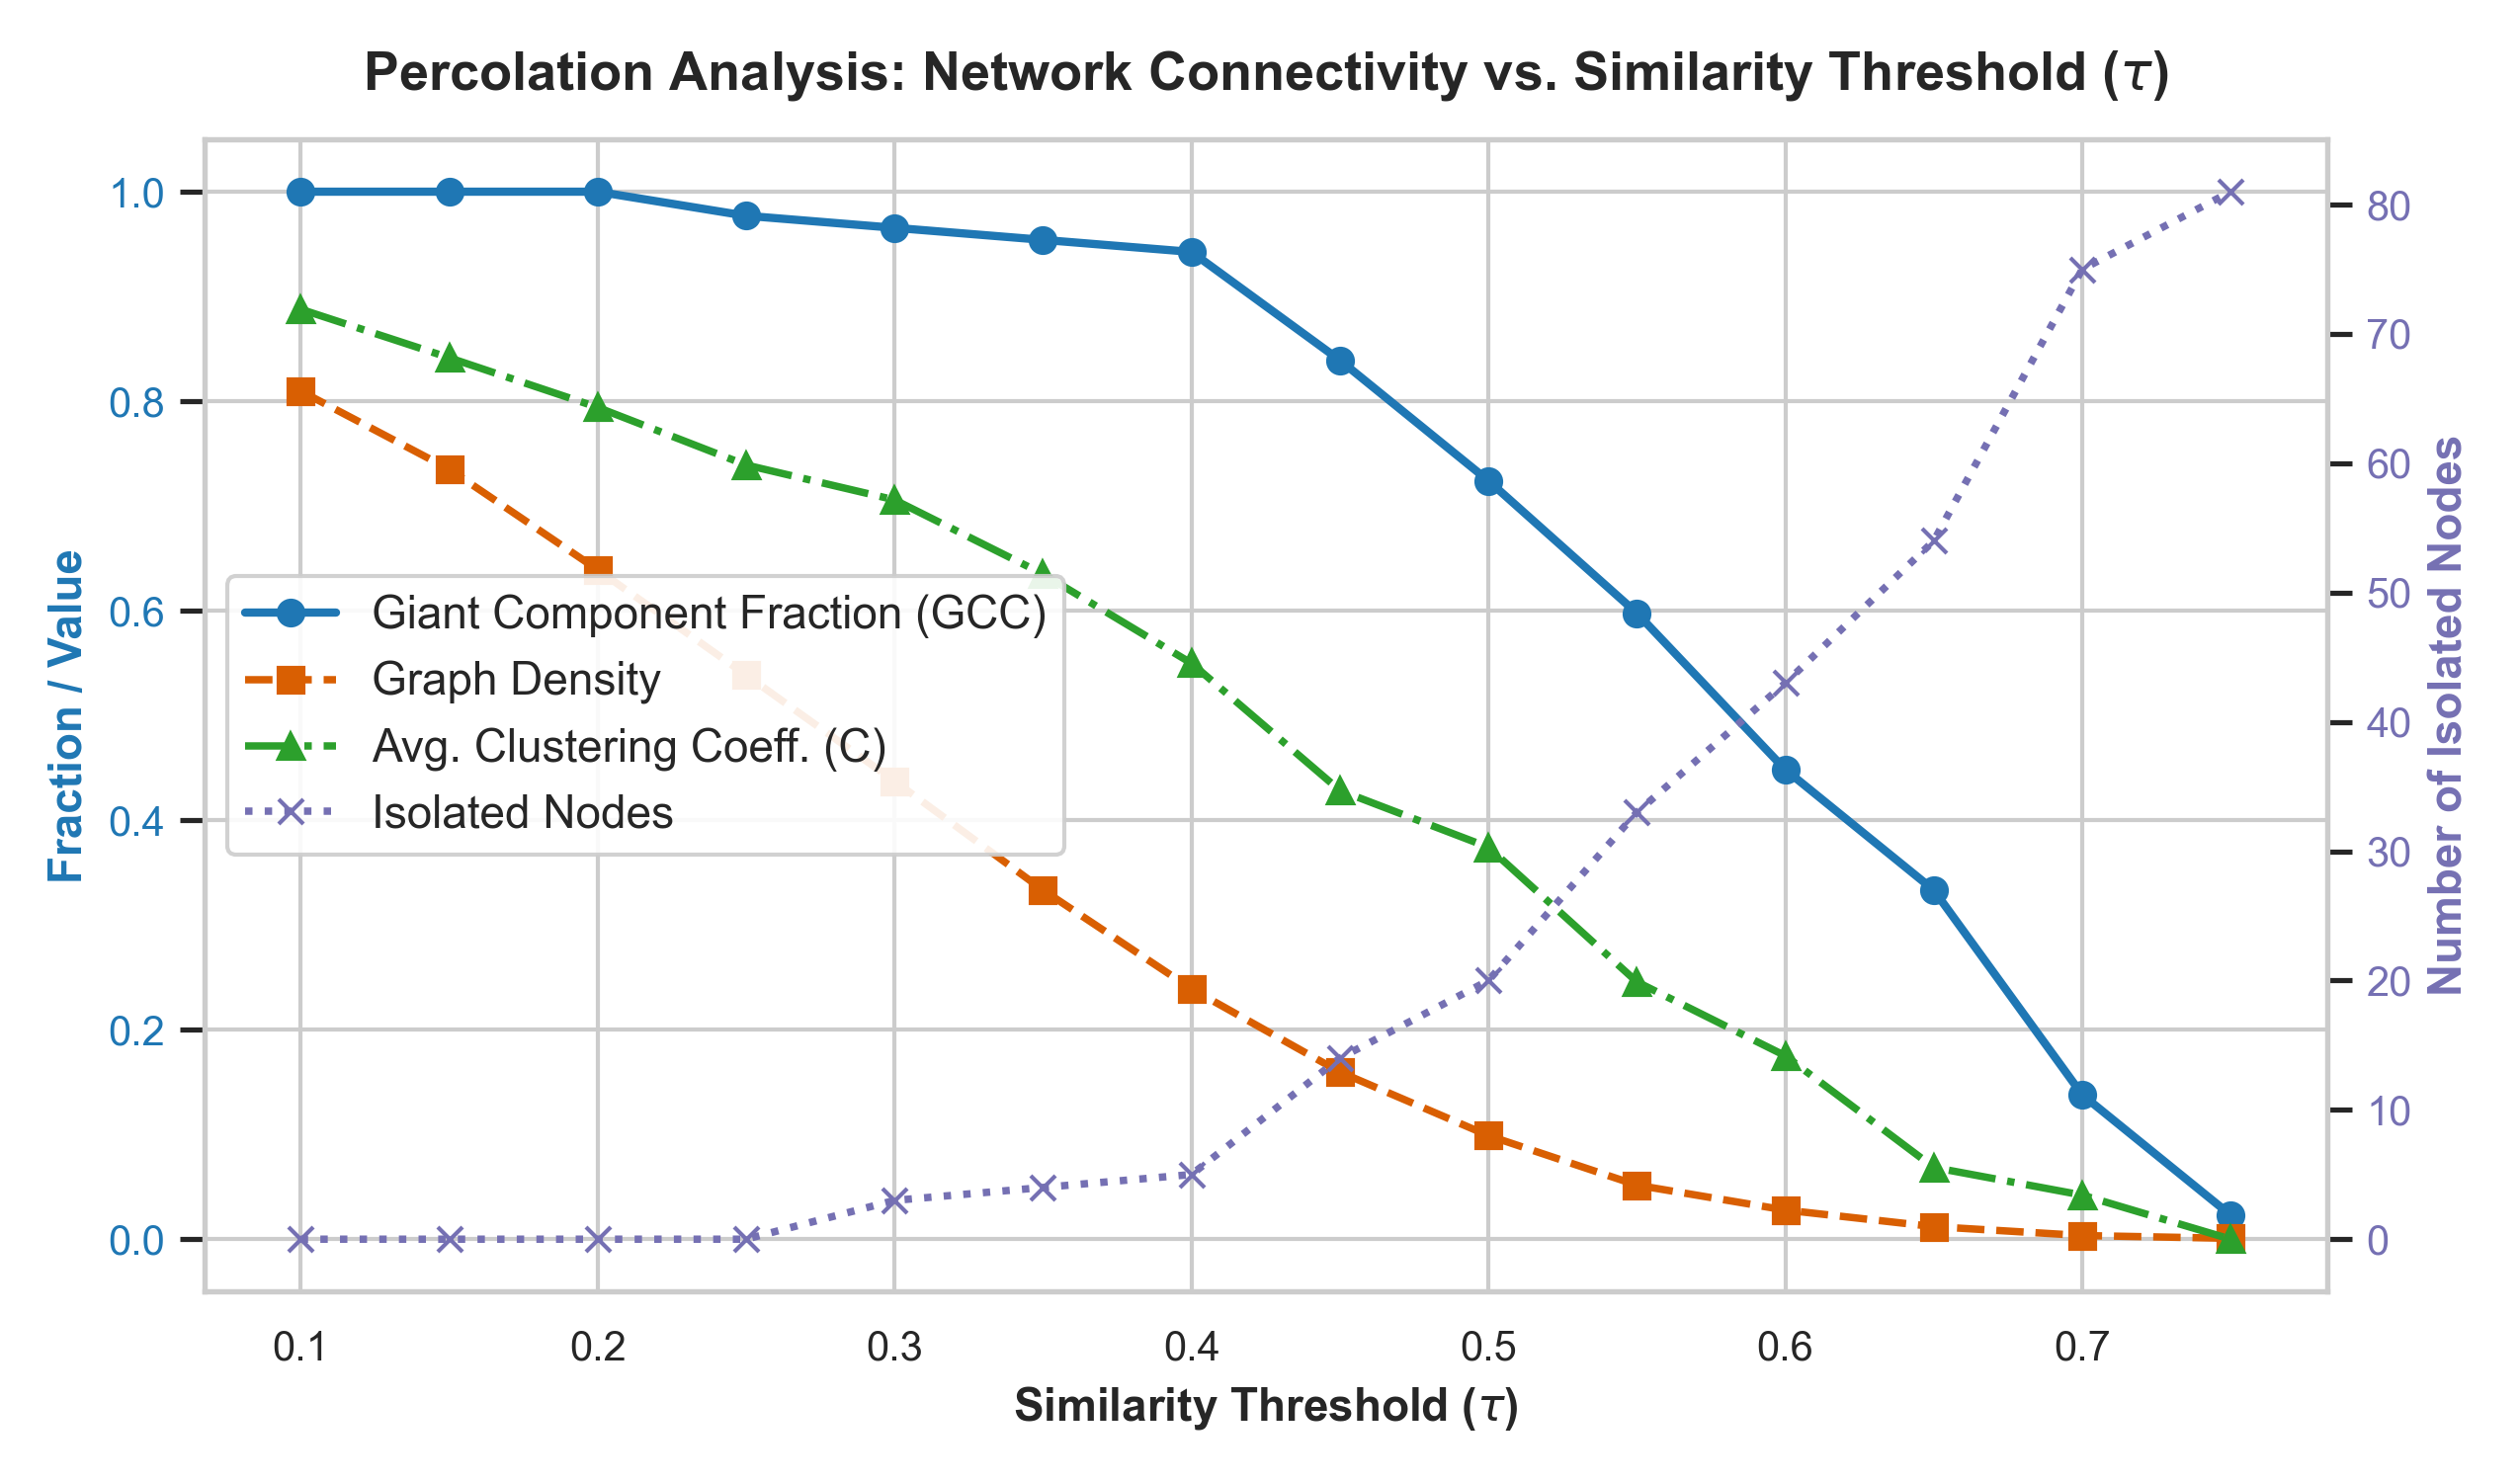
\includegraphics[width=\textwidth]{figures/fig1_percolation_analysis.png}
    \caption{Model 1: Student Network percolation sweep.}
    \label{fig:student_percolation}
\end{subfigure}
\hfill
\begin{subfigure}[b]{0.485\textwidth}
    \centering
    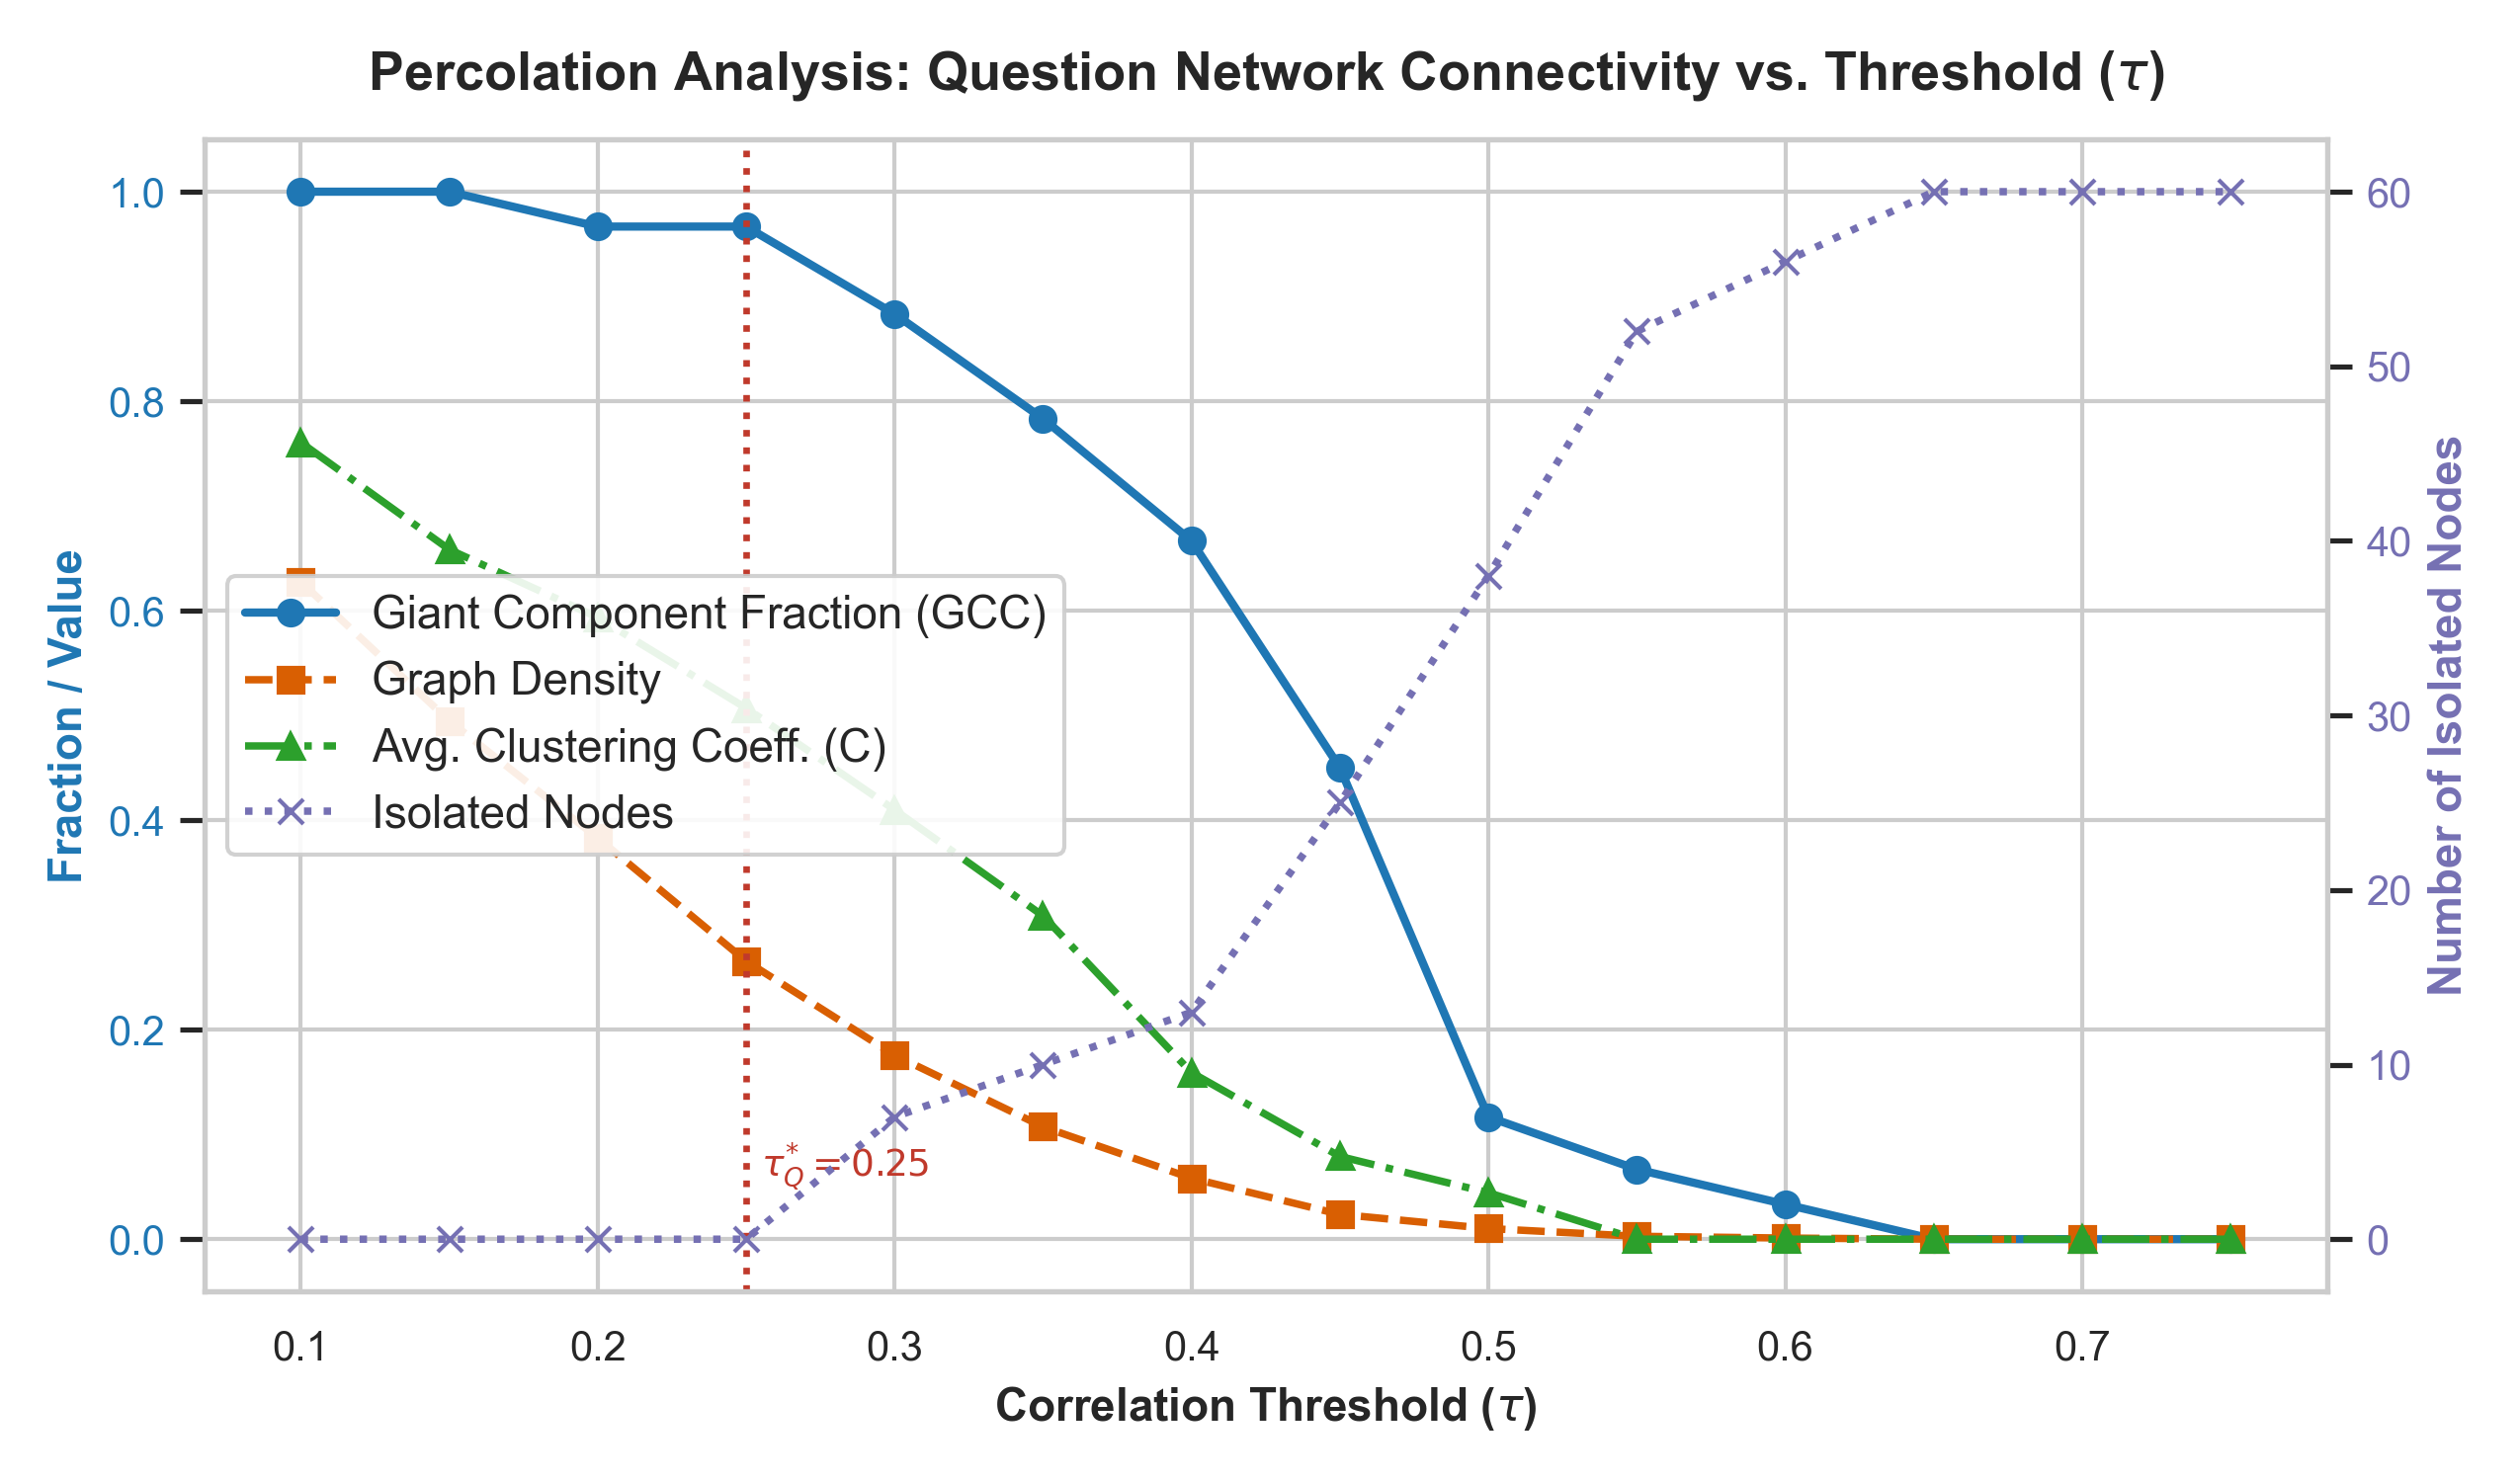
\includegraphics[width=\textwidth]{figures/fig7_question_percolation_analysis.png}
    \caption{Model 2: Question Network percolation sweep.}
    \label{fig:question_percolation}
\end{subfigure}
\caption{Percolation threshold parameter sweeps across $\tau \in [0.10, 0.75]$. Primary axes display GCC fraction, graph density, and average clustering coefficient; secondary axes display isolated node count. Selected cutoffs $\tau^*_S = 0.35$ and $\tau^*_Q = 0.25$ maximize network sparsity while preserving $\ge 95\%$ giant-component connectivity.}
\label{fig:percolation_both}
\end{figure*}

\subsection{Mathematical Network Formulations}

\subsubsection{\texorpdfstring{Model 1: Student Opinion Network ($G_S$)}{Model 1: Student Opinion Network (G\_S)}}
Let $V_S = \{s_1, \dots, s_N\}$ denote the $N = 87$ students, where each student $i$ is characterized by an opinion vector $\mathbf{v}_i \in \mathbb{R}^K$ ($K = 60$). Pairwise alignment is quantified via the sample \textbf{Pearson Correlation Coefficient}:
\begin{equation}
\label{eq:pearson_student}
r_{ij} = \frac{\sum_{k=1}^{K} (v_{ik} - \bar{v}_i)(v_{jk} - \bar{v}_j)}{\sqrt{\sum_{k=1}^{K} (v_{ik} - \bar{v}_i)^2} \sqrt{\sum_{k=1}^{K} (v_{jk} - \bar{v}_j)^2}} \in [-1, 1]
\end{equation}
where $\bar{v}_i = \frac{1}{K} \sum_{k=1}^K v_{ik}$. Applying cutoff $\tau^*_S$, binary adjacency matrix $A$ and weighted matrix $W$ are defined as:
\begin{align}
\label{eq:graph_adj_A}
A_{ij} &= \begin{cases} 
1 & \text{if } r_{ij} \ge \tau^*_S \text{ and } i \ne j \\ 
0 & \text{otherwise} 
\end{cases} \\
\label{eq:graph_adj_W}
W_{ij} &= \begin{cases} 
r_{ij} & \text{if } r_{ij} \ge \tau^*_S \text{ and } i \ne j \\ 
0 & \text{otherwise} 
\end{cases}
\end{align}
Self-loops are excluded ($A_{ii} = 0$). Negative correlations and sub-threshold positive alignments are mapped to non-edges.

\subsubsection{\texorpdfstring{Model 2: Question Concept Network ($G_Q$)}{Model 2: Question Concept Network (G\_Q)}}
Let $V_Q = \{q_1, \dots, q_K\}$ denote the 60 questions, represented by column vectors $\mathbf{q}_a \in \mathbb{R}^N$. Pairwise correlation is $r_{q_a, q_b} = \text{corr}(\mathbf{q}_a, \mathbf{q}_b)$. Edges exist if $r_{q_a, q_b} \ge \tau^*_Q$ ($a \ne b$), weighted by $W_{ab} = r_{q_a, q_b}$.

\subsection{Percolation Threshold Analysis}
We performed systematic percolation sweeps across $\tau \in [0.10, 0.75]$ with step size $\Delta \tau = 0.05$, tracking edges ($M$), density ($\rho$), Giant Connected Component fraction ($|V_{\text{GCC}}| / N$), isolates, and clustering ($C$).

\paragraph{Selection Rule:} Select the \textbf{largest threshold $\tau^*$ that preserves $\ge 95\%$ of nodes in the Giant Connected Component}.
\begin{itemize}[noitemsep,topsep=1pt,leftmargin=1.2em]
    \item \textbf{Student Network ($G_S$):} As shown in Figure~\ref{fig:student_percolation}, GCC coverage remains robust at $95.40\%$ (83/87 nodes, 4 isolates) at $\tau = 0.35$, while density drops to $\rho = 0.3333$ ($M = 1,247$, filtering $58.8\%$ of edges from $\tau = 0.10$). Above $\tau = 0.40$, fragmentation accelerates (GCC drops to $83.91\%$ at $\tau = 0.45$; isolates jump to 14). Thus, \textbf{$\tau^*_S = 0.35$} is selected.
    \item \textbf{Question Network ($G_Q$):} As shown in Figure~\ref{fig:question_percolation}, GCC coverage holds at $96.67\%$ (58/60 nodes) through $\tau = 0.25$ before falling to $88.33\%$ at $\tau = 0.30$ and $78.33\%$ at $\tau = 0.35$. Thus, \textbf{$\tau^*_Q = 0.25$} ($M = 470, \rho = 0.2655$) is the percolation-justified threshold.
\end{itemize}

% --- Pre-queue Table 1 so it appears cleanly at the top of Page 4 ---
\begin{table*}[t]
\centering
\small
\caption{Global topological properties of the empirical Student Opinion Network ($G_S$) at percolation threshold $\tau^*_S = 0.35$, benchmarked against an ensemble of 50 Erd\H{o}s--R\'enyi $G(N, p)$ random graphs and theoretical expectations.}
\label{tab:global_metrics}
\resizebox{\textwidth}{!}{%
\begin{tabular}{lcccc}
\toprule
\textbf{Metric} & \textbf{Empirical Network ($G_S$)} & \textbf{ER Baseline (Simulated, $N=50$)} & \textbf{Theoretical ER} & \textbf{Ratio / Significance} \\
\midrule
Number of Nodes ($N$) & 87 & 87 & 87 & Exact match \\
Number of Edges ($M$) & 1,247 & $1,247 \pm 28.5$ & --- & Exact match \\
Average Degree ($\langle k \rangle$) & 28.667 & $28.667 \pm 0.655$ & $p(N-1) = 28.667$ & Exact match \\
Graph Density ($\rho$) & 0.3333 & $0.3333 \pm 0.0076$ & $p = 0.3333$ & Exact match \\
Clustering Coefficient ($C$) & \textbf{0.6350} & \textbf{0.3340 $\pm$ 0.0077} & $p = 0.3333$ & $\gamma = C / C_{\text{ER}} = 1.9015$ ($z \approx 39.1$) \\
Network Transitivity & 0.6500 & $0.3339 \pm 0.0075$ & $p = 0.3333$ & $1.9467\times$ ER baseline \\
GCC Node Count & 83 (95.40\%) & $87.0 \pm 0.0$ (100\%) & --- & 4 peripheral isolates \\
Connected Components & 5 & $1.0 \pm 0.0$ & --- & 1 GCC + 4 singletons \\
Avg. Path Length GCC ($L$) & \textbf{1.7161} & \textbf{1.6669 $\pm$ 0.0074} & $\frac{\ln N}{\ln \langle k \rangle} = 1.3308$ & $\lambda = L / L_{\text{ER}} = 1.0295$ \\
Graph Diameter (GCC) & 4 & $2.0 \pm 0.0$ & --- & Worst-case geodesic \\
Degree Assortativity ($r$) & -0.0199 & $0.0012 \pm 0.0241$ & 0.0 & Weakly disassortative \\
Louvain Modularity ($Q$) & 0.1293 & --- & --- & 4 primary communities \\
\textbf{Small-World Index ($\sigma$)} & \textbf{1.8469} & 1.0000 & 1.0000 & $\sigma = \gamma / \lambda > 1$ \\
\bottomrule
\end{tabular}%
}
\end{table*}


\subsection{Topological Metrics and Null Model Benchmarking}
We compute standard network metrics:
\begin{itemize}[noitemsep,topsep=1pt,leftmargin=1.2em]
    \item \textbf{Degree Centrality ($C_D$):} $C_D(i) = \frac{k_i}{N - 1} = \frac{1}{N - 1}\sum_{j \ne i} A_{ij}$.
    \item \textbf{Betweenness Centrality ($C_B$):} $C_B(i) = \sum_{s \ne i \ne t} \frac{\sigma_{st}(i)}{\sigma_{st}}$.
    \item \textbf{Closeness Centrality ($C_C$):} $C_C(i) = \frac{N - 1}{\sum_{j \ne i} d(i, j)}$.
    \item \textbf{Local Clustering ($C_i$):} $C_i = \frac{2 e_i}{k_i(k_i - 1)} = \frac{\sum_{j, k} A_{ij} A_{jk} A_{ki}}{k_i(k_i - 1)}$.
    \item \textbf{Erd\H{o}s--R\'enyi $G(N, p)$ Baseline:} Benchmark $G_S$ against an ensemble of 50 simulated random graphs ($N = 87, p = 0.3333$).
    \item \textbf{Small-World Index ($\sigma$):} Following Watts-Strogatz and Humphries-Gurney:
    \begin{equation}
    \label{eq:small_world}
    \gamma = \frac{C_{\text{empirical}}}{C_{\text{ER}}^{\text{simulated}}}, \quad \lambda = \frac{L_{\text{empirical}}}{L_{\text{ER}}^{\text{simulated}}}, \quad \sigma = \frac{\gamma}{\lambda}
    \end{equation}
    A network exhibits small-world organization when $\gamma > 1$ and $\lambda \approx 1$, yielding $\sigma > 1$.
\end{itemize}

% ==============================================================================
% SECTION 5: ANALYSIS AND VISUALIZATIONS
% ==============================================================================
\section{Analysis and Visualizations}
\label{sec:analysis}

\subsection{Global Properties and Random Benchmarking}
Table~\ref{tab:global_metrics} compares $G_S$ against the 50-run Erd\H{o}s--R\'enyi ensemble.

Key measured findings include:
\begin{itemize}[noitemsep,topsep=1pt,leftmargin=1.2em]
    \item \textbf{Clustering Elevation ($\gamma = 1.9015$):} The empirical clustering ($C = 0.6350$) is nearly double the random null model ($C_{\text{ER}} = 0.3340 \pm 0.0077, z \approx 39.1$).
    \item \textbf{Geodesic Path Parity ($\lambda = 1.0295$):} Empirical GCC path length ($L = 1.7161$) matches the random baseline ($L_{\text{ER}} = 1.6669 \pm 0.0074$) within $3.0\%$.
    \item \textbf{Small-World Index ($\sigma = 1.8469$):} With $\gamma = 1.9015 > 1$ and $\lambda = 1.0295 \approx 1$, $\sigma = 1.8469$ confirms small-world properties relative to ER random graphs.
    \item \textbf{Degree Assortativity ($r = -0.0199$):} Near-zero correlation indicates that consensus hubs connect broadly across high- and low-degree peers rather than forming an isolated core.
\end{itemize}

\subsection{Degree Distribution vs. Poisson Null Model}
Figure~\ref{fig:degree_dist} contrasts empirical degrees against the theoretical Poisson fit ($\lambda = 28.7$).

\begin{figure}[h]
\centering
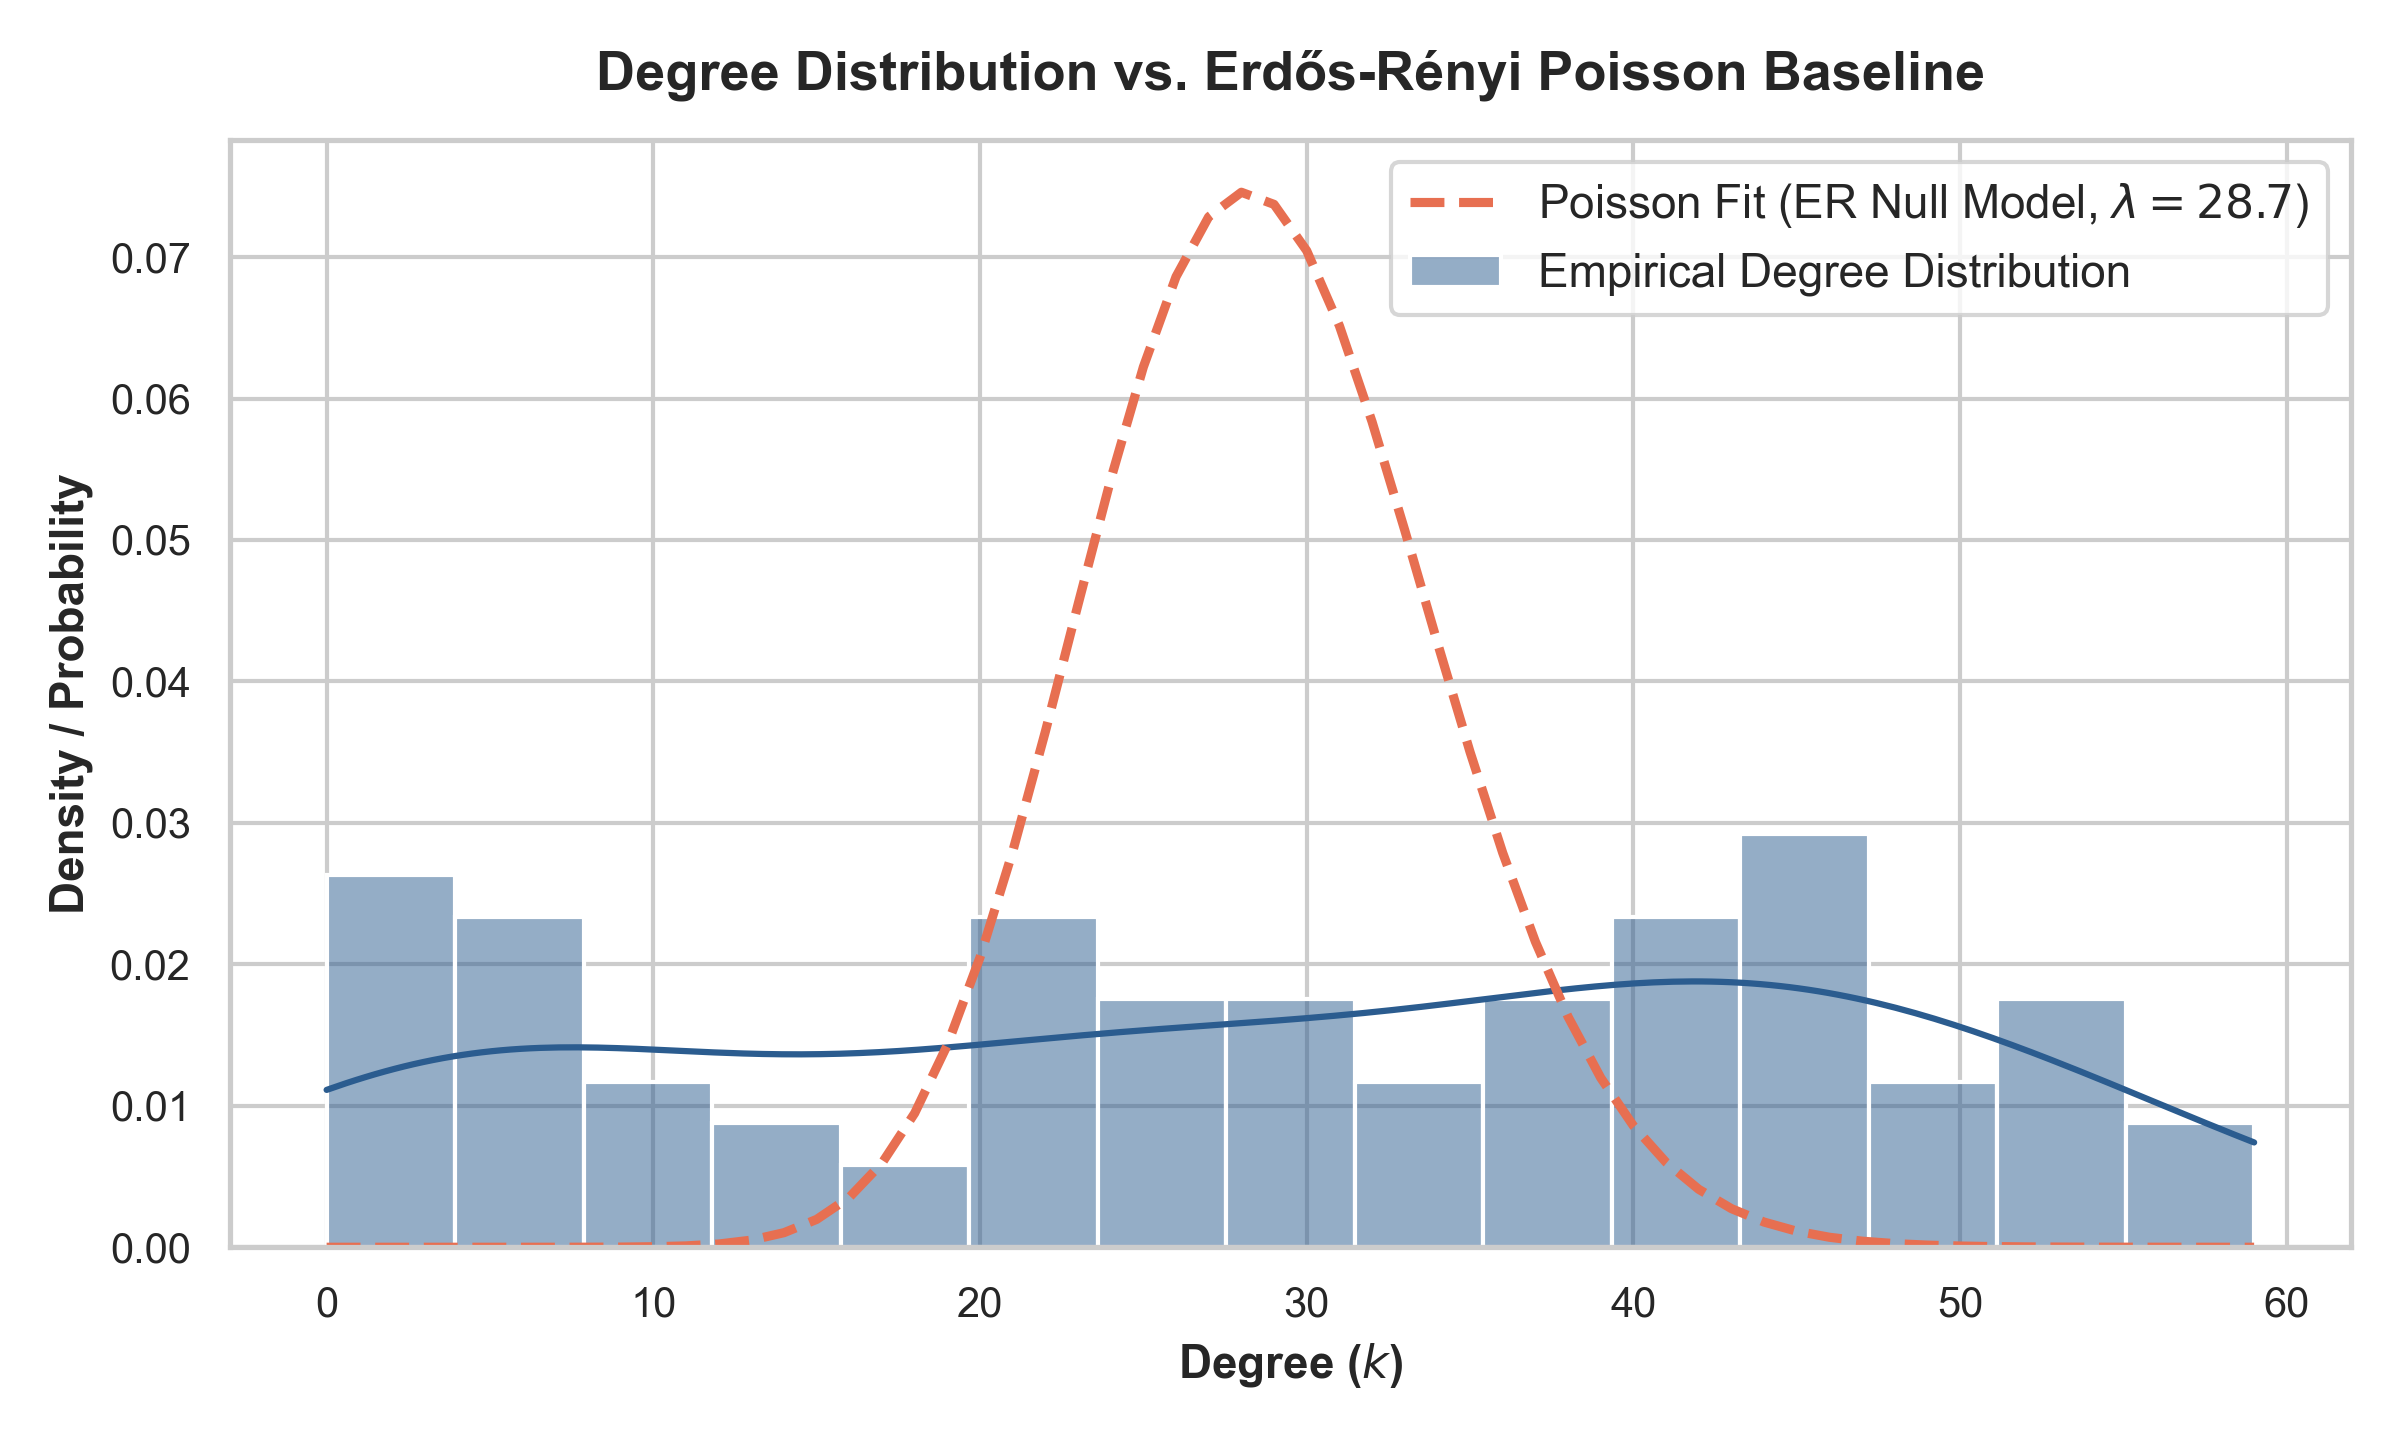
\includegraphics[width=\columnwidth]{figures/fig3_degree_distribution.png}
\caption{Degree distribution of $G_S$ vs. theoretical Poisson fit ($\lambda = 28.7$) of the Erd\H{o}s--R\'enyi baseline, showing high variance and positive skew.}
\label{fig:degree_dist}
\end{figure}

The empirical distribution displays high variance ($\approx 208.4$) compared to the Poisson baseline ($\text{variance} = \lambda = 28.7$). The right-skewed tail reflects consensus hubs connected to $>65\%$ of peers, alongside peripheral isolates.

\subsection{Consensus Hubs vs. Structural Bridges}
Table~\ref{tab:student_centralities} lists the top ranking respondents by Degree ($C_D$) and Betweenness ($C_B$).

\begin{table}[t]
\centering
\small
\caption{Top ranking respondents in the Student Opinion Network ($G_S$) classified by Degree Centrality (consensus hubs) and Betweenness Centrality (topological bridges).}
\label{tab:student_centralities}
\resizebox{\columnwidth}{!}{%
\begin{tabular}{ccccccc}
\toprule
\textbf{ID} & \textbf{Degree} & $C_D$ & \textbf{Strength} & $C_B$ & $C_C$ & \textbf{Comm.} \\
\midrule
\multicolumn{7}{l}{\textbf{Top 5 Consensus Hubs (Degree Centrality)}} \\
114 & 59 & 0.6860 & 30.327 & 0.0288 & 0.7446 & Comm 3 \\
55  & 58 & 0.6744 & 28.125 & 0.0192 & 0.7376 & Comm 1 \\
61  & 56 & 0.6512 & 28.831 & 0.0164 & 0.7173 & Comm 4 \\
49  & 55 & 0.6395 & 28.448 & 0.0166 & 0.7173 & Comm 4 \\
70  & 55 & 0.6395 & 26.564 & 0.0255 & 0.7108 & Comm 1 \\
\midrule
\multicolumn{7}{l}{\textbf{Top 5 Topological Bridges (Betweenness Centrality)}} \\
90  & 52 & 0.6047 & 26.466 & \textbf{0.0346} & 0.6919 & Comm 2 \\
19  & 41 & 0.4767 & 18.260 & \textbf{0.0307} & 0.6305 & Comm 1 \\
53  & 48 & 0.5581 & 22.841 & \textbf{0.0290} & 0.6626 & Comm 2 \\
114 & 59 & 0.6860 & 30.327 & \textbf{0.0288} & 0.7446 & Comm 3 \\
41  & 35 & 0.4070 & 16.148 & \textbf{0.0264} & 0.5923 & Comm 2 \\
\bottomrule
\end{tabular}%
}
\end{table}


\begin{itemize}[noitemsep,topsep=1pt,leftmargin=1.2em]
    \item \textbf{Consensus Hubs:} Student \texttt{114} achieves the highest degree ($k = 59, C_D = 0.6860$, Closeness $0.7446$), followed by Student \texttt{55} ($k = 58$) and Student \texttt{61} ($k = 56$).
    \item \textbf{Topological Bridges:} Student \texttt{90} exhibits the highest betweenness ($C_B = 0.0346, k=52$), followed by Student \texttt{19} ($C_B = 0.0307, k=41$) and Student \texttt{53} ($C_B = 0.0290, k=48$). Student \texttt{114} ranks fourth in betweenness ($0.0288$) while leading in degree.
\end{itemize}

% --- Pre-queue Figure 4 so it appears cleanly at the top of Page 5 ---
\begin{figure*}[t]
\centering
\begin{subfigure}[b]{0.485\textwidth}
    \centering
    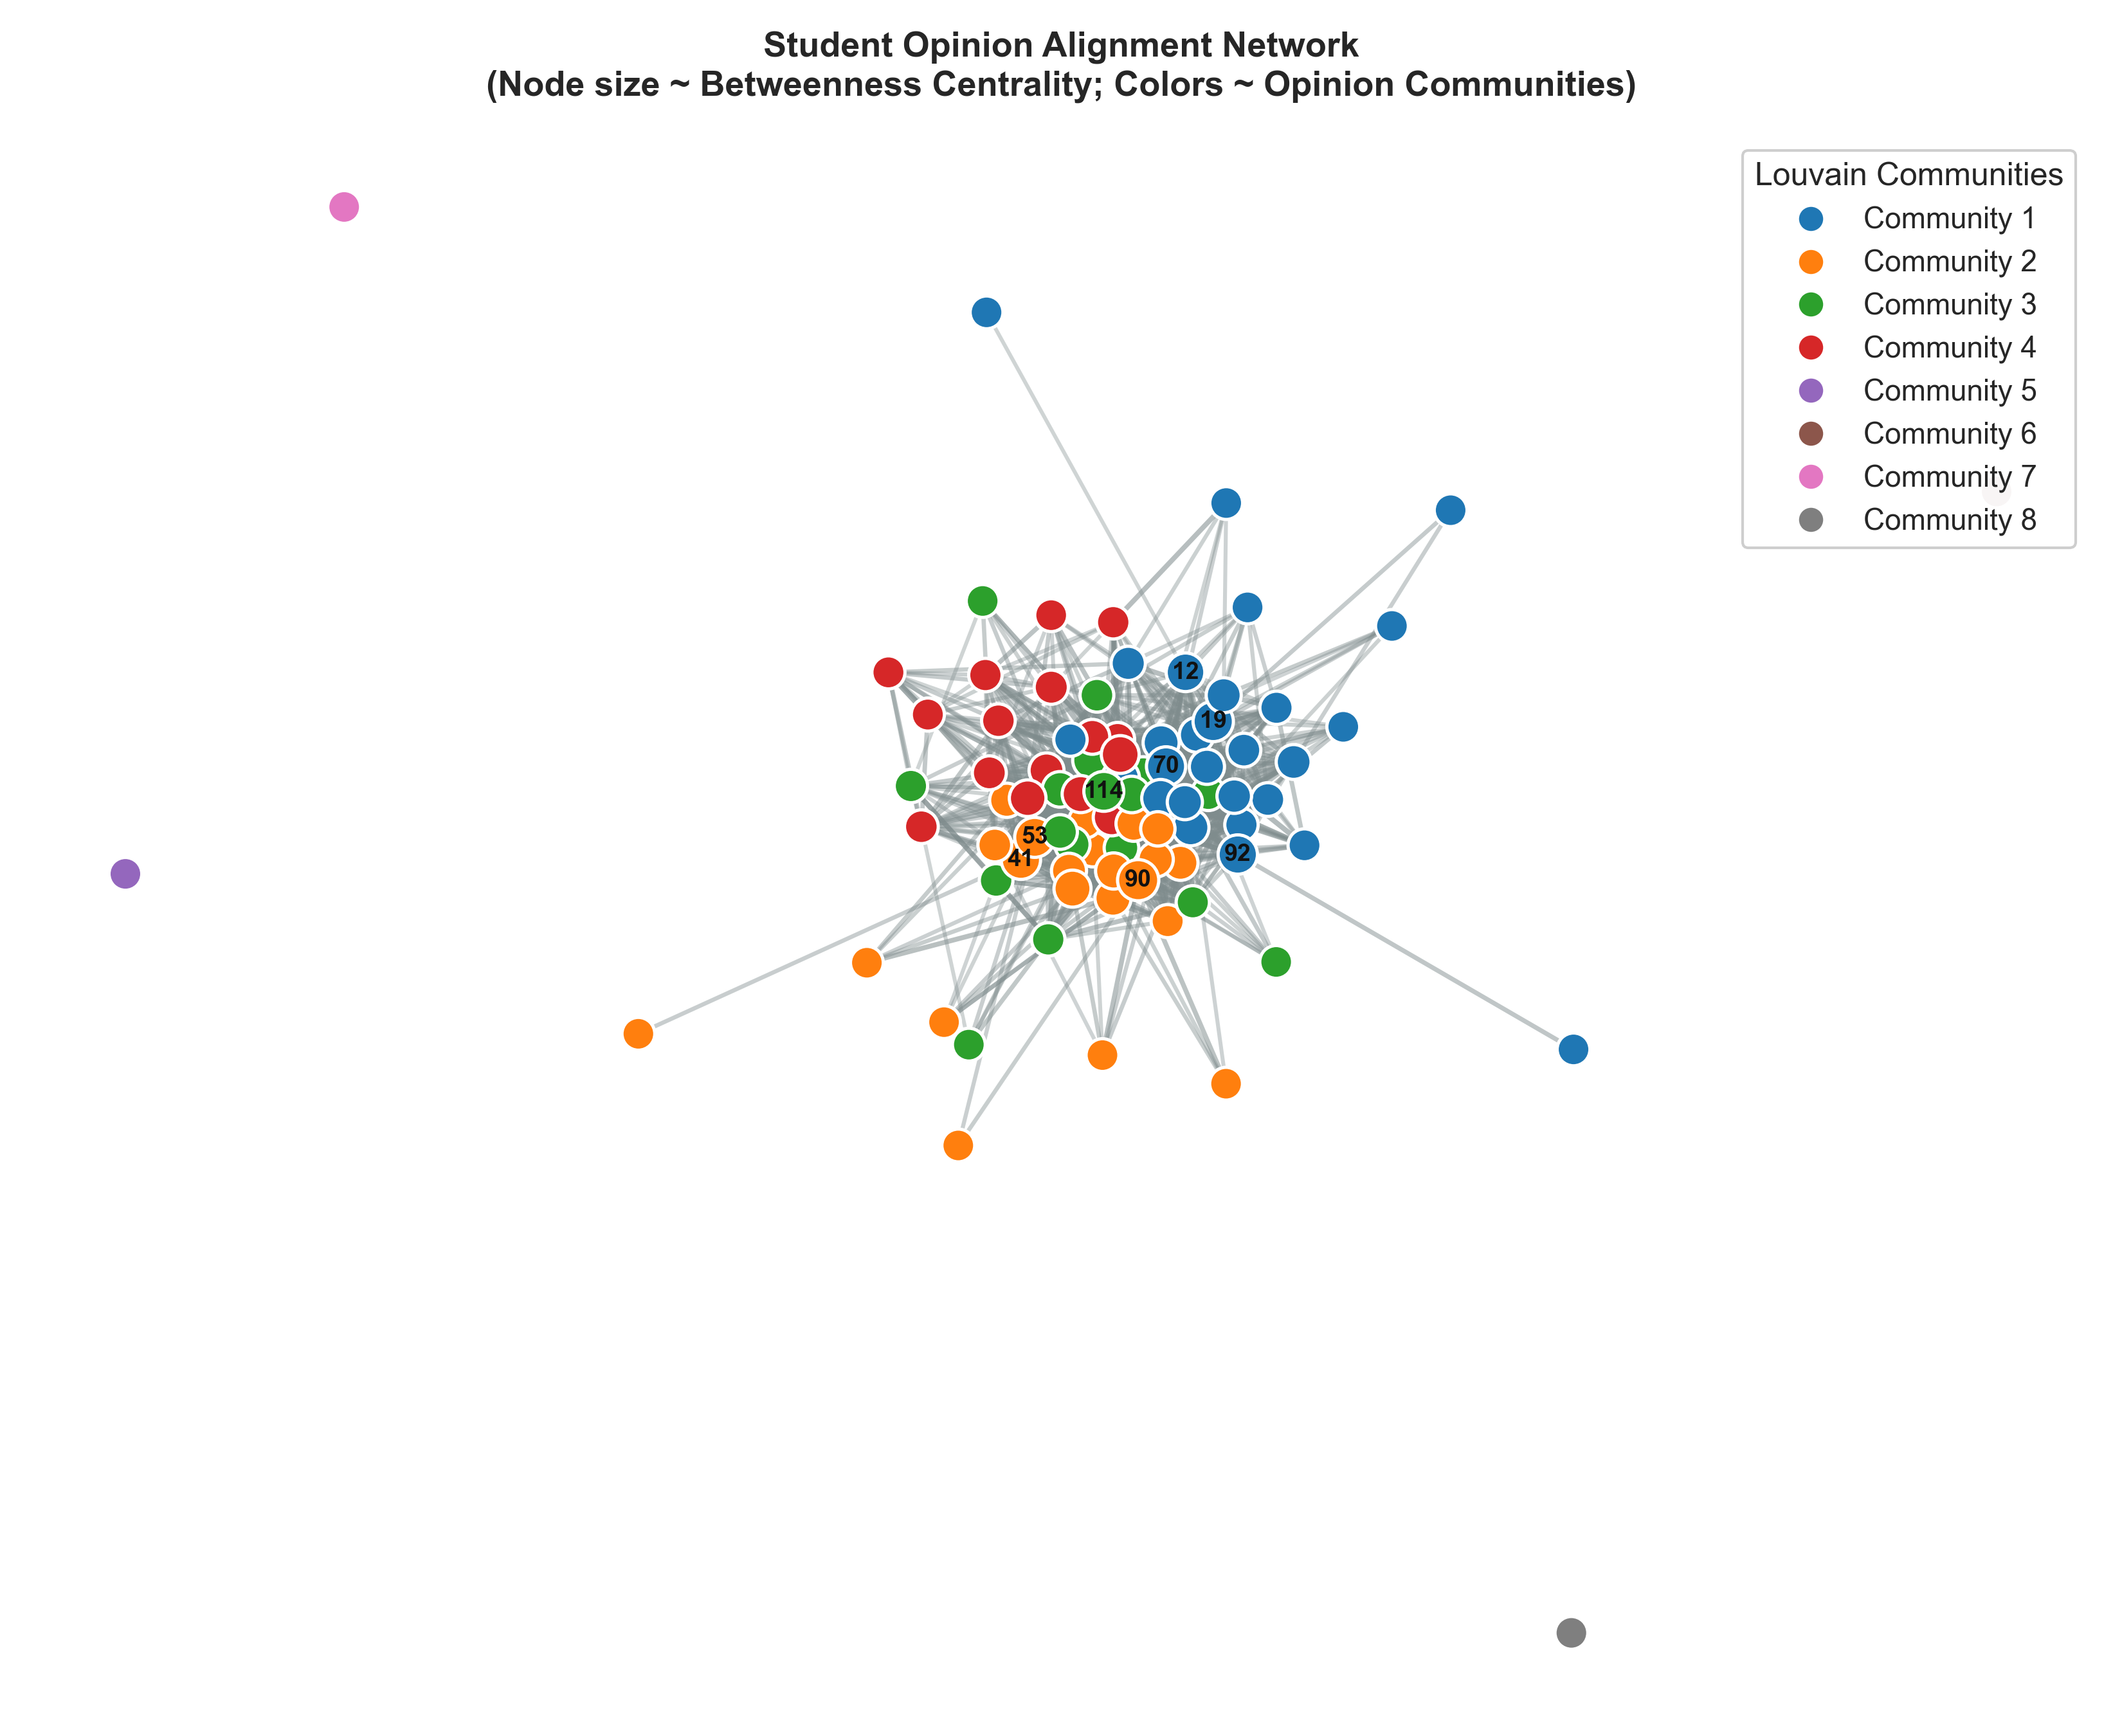
\includegraphics[width=\textwidth]{figures/fig2_student_network_communities.png}
    \caption{Student Opinion Network ($G_S$) Spring layout.}
    \label{fig:student_communities}
\end{subfigure}
\hfill
\begin{subfigure}[b]{0.485\textwidth}
    \centering
    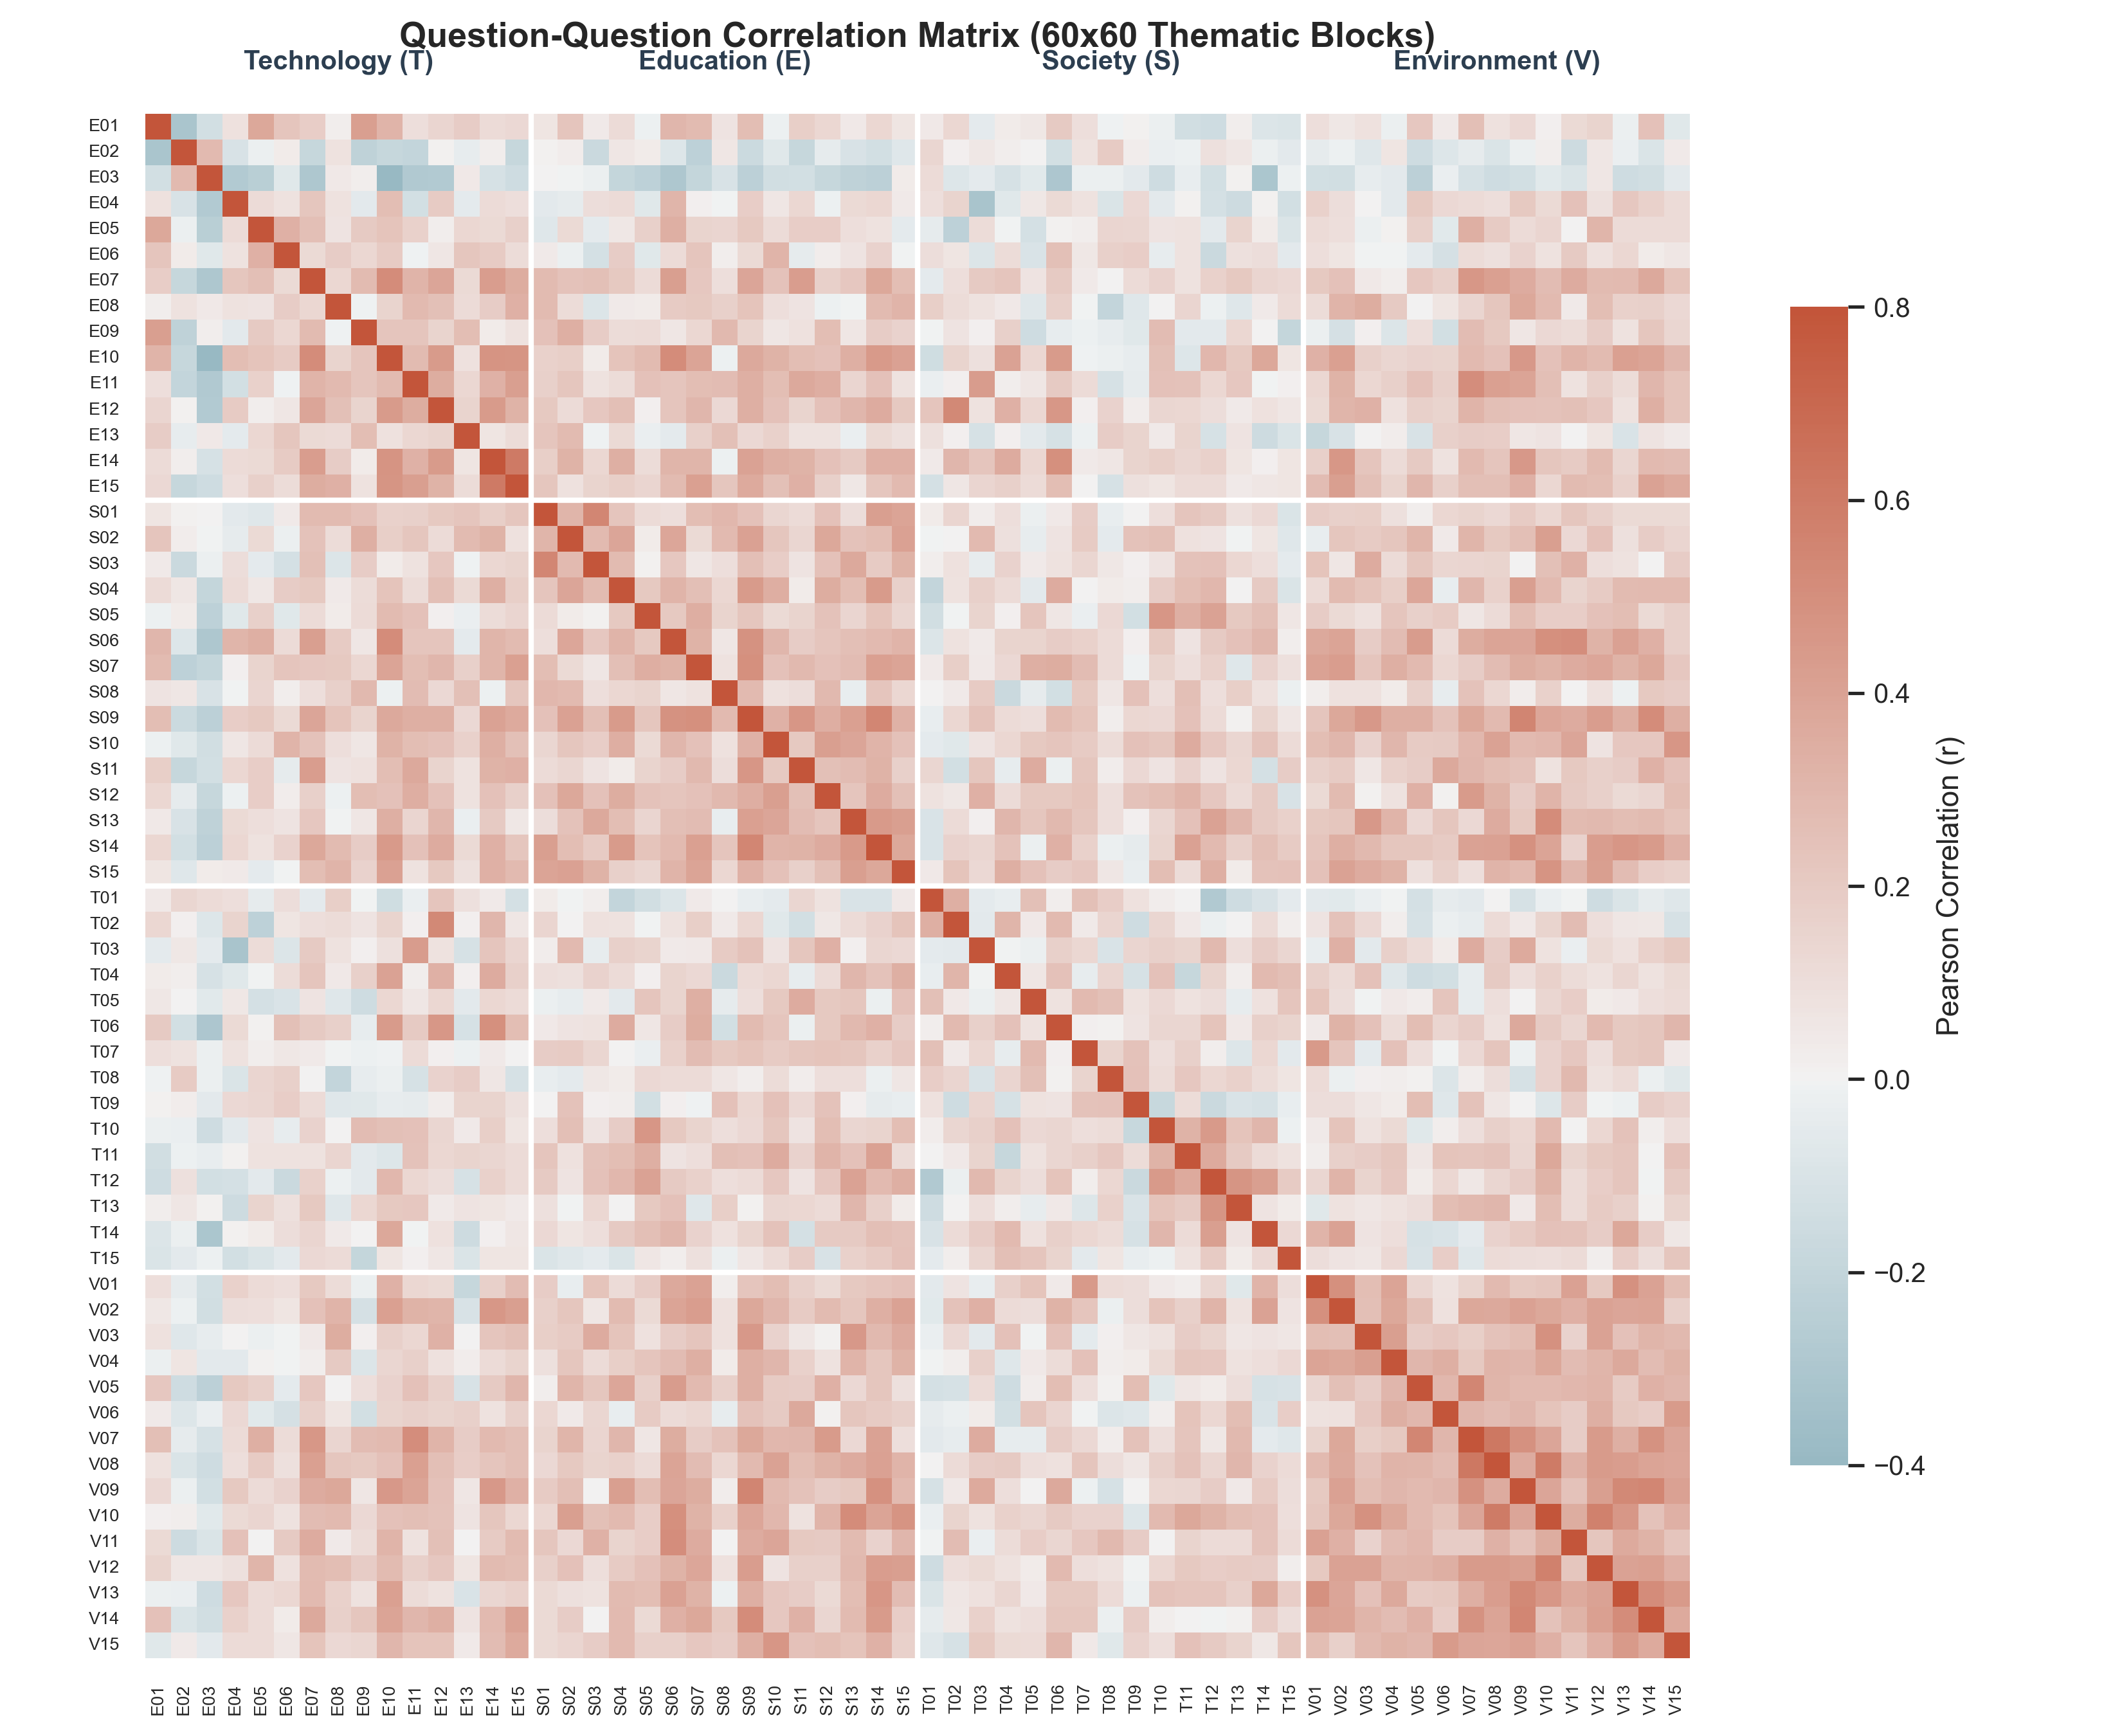
\includegraphics[width=\textwidth]{figures/fig5_question_correlation_heatmap.png}
    \caption{$60 \times 60$ Question Thematic Correlation Heatmap.}
    \label{fig:question_heatmap}
\end{subfigure}
\caption{Visual topology: (a) Student Opinion Network ($N=87, \tau^*_S = 0.35$) with nodes colored by Louvain community and sized by betweenness centrality; (b) Symmetric $60 \times 60$ correlation matrix partitioned into 15-question thematic blocks ($T, E, S, V$).}
\label{fig:visualizations_mid}
\end{figure*}

\subsection{Network Topology and Correlation Structure}
Figure~\ref{fig:student_communities} illustrates the force-directed layout of $G_S$, colored by Louvain community with node sizes scaled by betweenness. The four dominant communities form cohesive clusters surrounding central bridge nodes.

Figure~\ref{fig:question_heatmap} displays the $60 \times 60$ question correlation matrix. Strong positive correlation blocks appear in \textbf{Environment ($V$)} and \textbf{Society ($S$)}, while \textbf{Education ($E$)} exhibits lower internal correlation, reflecting heterogeneous sub-topics.

% ==============================================================================
% SECTION 6: RESULTS AND DISCUSSION
% ==============================================================================
\section{Results and Discussion}
\label{sec:results}

% --- Pre-queue Table 3 so it appears cleanly at the top of Page 6 ---
\begin{table*}[t]
\centering
\small
\caption{Louvain community structure ($Q = 0.1293$) and thematic mean response profiles across the four survey domains (Scale: $-2.0$ to $+2.0$).}
\label{tab:community_profiles}
\resizebox{\textwidth}{!}{%
\begin{tabular}{ccccccccc}
\toprule
\textbf{Community ID} & \textbf{Size ($N$)} & \textbf{Share (\%)} & \textbf{Tech ($T$)} & \textbf{Edu ($E$)} & \textbf{Society ($S$)} & \textbf{Env ($V$)} & \textbf{Overall Stance} & \textbf{Ideological Persona Characterization} \\
\midrule
\textbf{1} & 28 & 32.2\% & +0.874 & +1.029 & +1.207 & +1.369 & +1.120 & \textbf{Progressive Institutionalists:} Balanced; pro-ethics/environment. \\
\textbf{2} & 22 & 25.3\% & +1.036 & +1.033 & +1.473 & +1.412 & +1.239 & \textbf{Civic \& Environmental Champions:} Highest overall agreement. \\
\textbf{3} & 17 & 19.5\% & +1.173 & +0.773 & +1.192 & +1.455 & +1.148 & \textbf{Techno-Optimists:} Strong AI endorsement; critical of edu mandates. \\
\textbf{4} & 16 & 18.4\% & +0.996 & +0.787 & +1.350 & +1.508 & +1.160 & \textbf{Eco-Centric Reformers:} Highest environmental priority. \\
\midrule
\textbf{5 (ID 40)} & 1 & 1.1\% & +1.133 & +1.133 & +1.667 & +1.733 & +1.417 & \textbf{Singleton Isolate:} Uniformly high positive responses. \\
\textbf{6 (ID 119)} & 1 & 1.1\% & +0.800 & 0.000 & +0.067 & +0.200 & +0.267 & \textbf{Singleton Isolate:} Neutral on education and society. \\
\textbf{7 (ID 120)} & 1 & 1.1\% & -0.400 & -0.133 & 0.000 & -0.267 & -0.200 & \textbf{Singleton Isolate:} Cohort dissenter (negative overall stance). \\
\textbf{8 (ID 125)} & 1 & 1.1\% & +1.200 & +0.333 & +0.667 & +0.533 & +0.683 & \textbf{Singleton Isolate:} Moderate idiosyncratic profile. \\
\bottomrule
\end{tabular}%
}
\end{table*}


\subsection{Community Structure and Thematic Personas}
Applying weighted Louvain modularity optimization on $G_S$ (\texttt{seed=42}) yields modularity $Q = 0.1293$, partitioning the cohort into \textbf{four primary opinion communities} ($95.40\%$ of students) plus \textbf{four singleton isolates} (Table~\ref{tab:community_profiles} and Figure~\ref{fig:community_question_analysis}a).

To establish a comprehensive understanding of opinion organization, we conduct a multi-scale analysis combining \textbf{group-level community opinion profiles} (Figure~\ref{fig:community_question_analysis}a) with \textbf{item-level question response dispersion} (Figure~\ref{fig:community_question_analysis}b). While community profiling identifies how structurally partitioned sub-cohorts systematically diverge in their domain-level philosophies (e.g., Techno-Optimists vs. Eco-Centric Reformers), question-wise variance isolates the specific pedagogical and socio-technical policy statements that trigger polarization versus universal consensus across the student body.

\begin{figure*}[t]
\centering
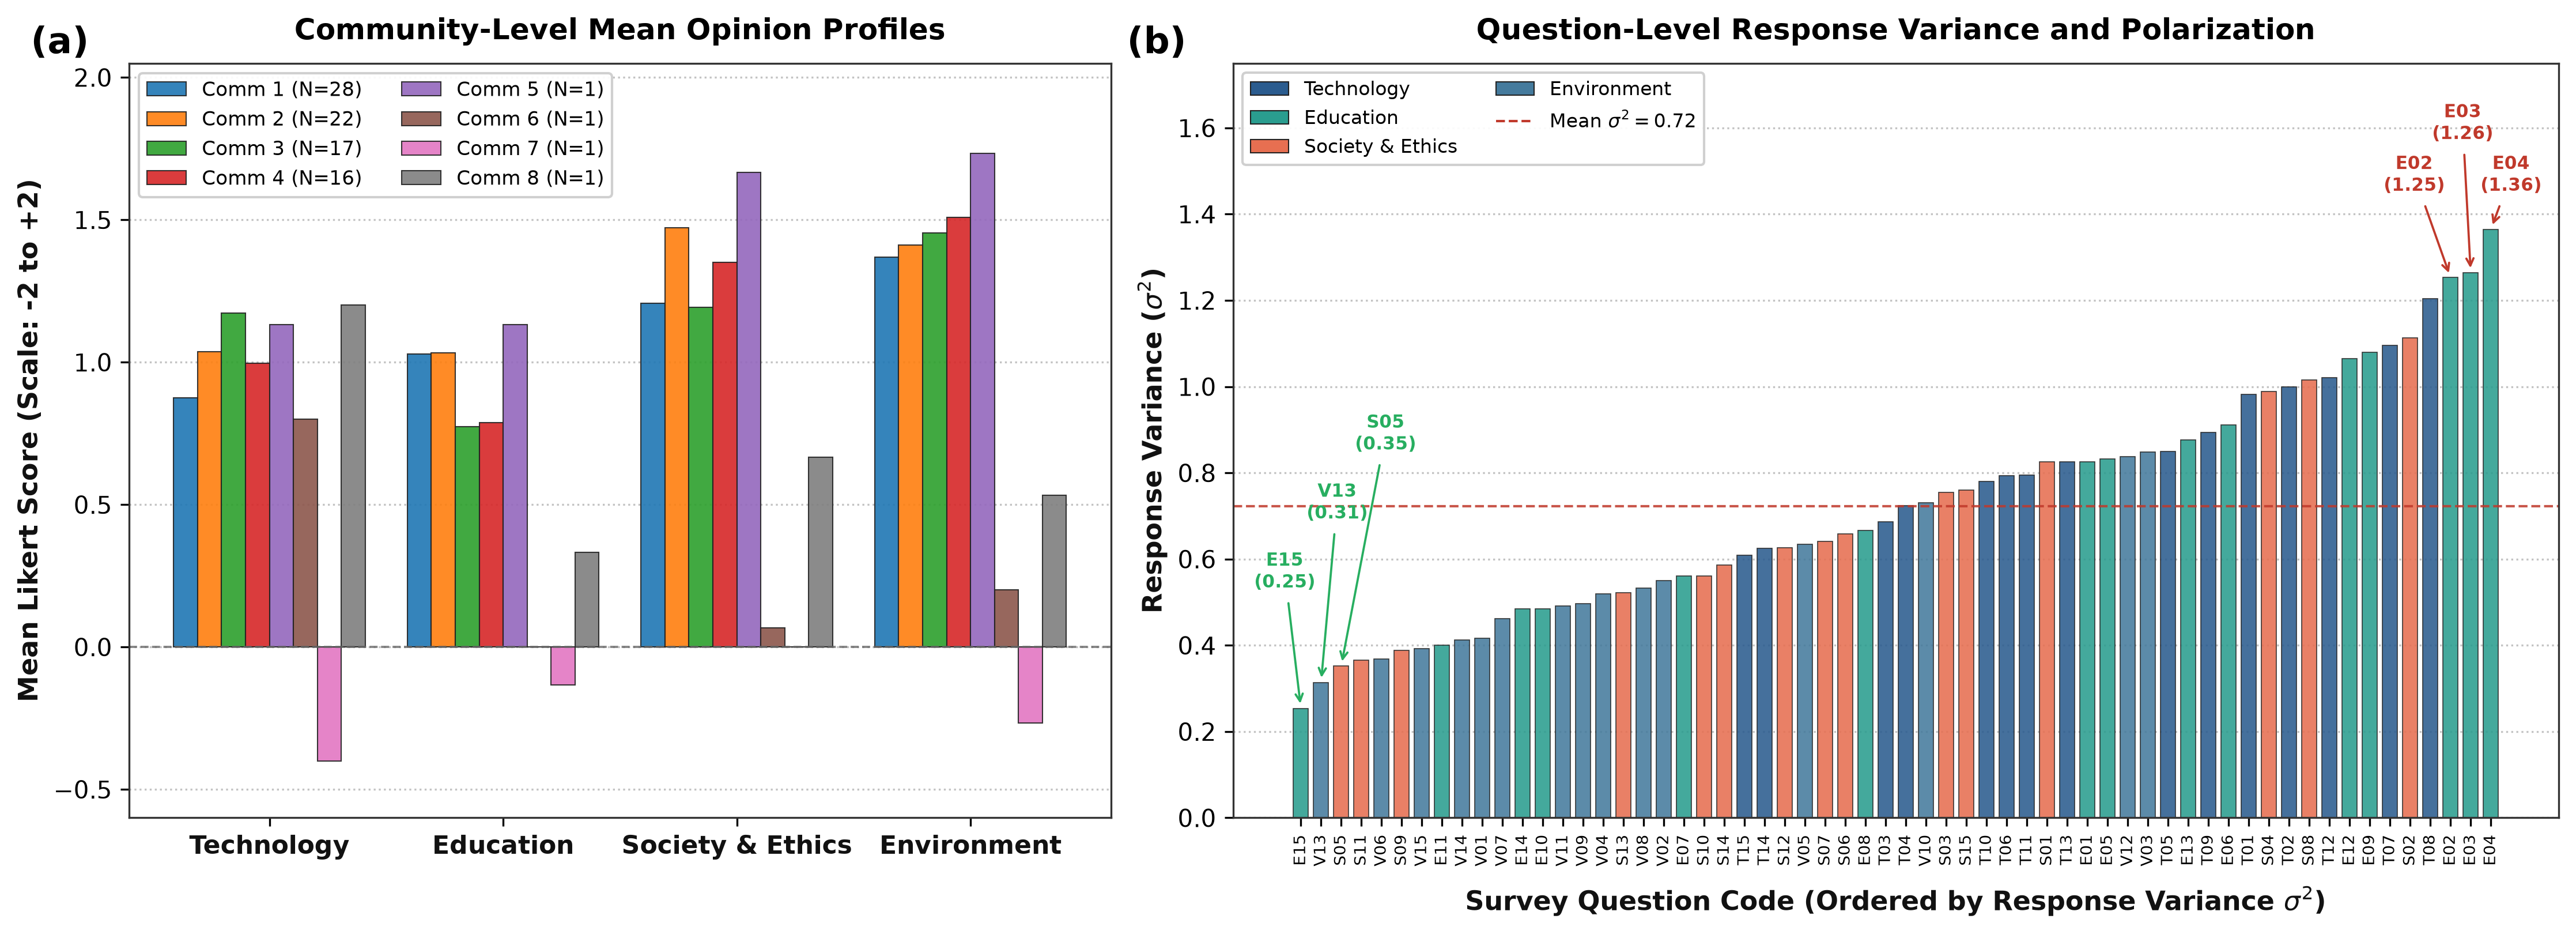
\includegraphics[width=\textwidth]{figures/fig5_community_and_question_polarization.png}
\caption{Community-level and question-level opinion structure. (a) Mean Likert response profiles across Technology, Education, Society \& Ethics, and Environment for the Louvain communities identified in the Student Opinion Network. (b) Question-wise response variance across all 60 survey questions (ordered by variance), with higher variance indicating greater disagreement within the cohort. The most divisive questions are concentrated in the Education domain, while the lowest-variance questions indicate stronger cohort consensus.}
\label{fig:community_question_analysis}
\label{fig:community_radar}
\end{figure*}

\paragraph{Ideological Personas:}
\begin{enumerate}[noitemsep,topsep=1pt,leftmargin=1.2em]
    \item \textbf{Community 1: Progressive Institutionalists ($N = 28, 32.2\%$):} Balanced stance ($+1.120$ overall), supporting environmental mandates ($+1.369$) and structured educational reform ($+1.029$).
    \item \textbf{Community 2: Civic Champions ($N = 22, 25.3\%$):} Highest overall agreement ($+1.239$), with strong conviction in ethics ($+1.473$) and sustainability ($+1.412$).
    \item \textbf{Community 3: Techno-Optimists ($N = 17, 19.5\%$):} Strongest AI endorsement ($+1.173$), but critical of educational mandates ($+0.773$).
    \item \textbf{Community 4: Eco-Centric Reformers ($N = 16, 18.4\%$):} Highest environmental conviction ($+1.508$), prioritizing sustainability over tech disruption ($+0.996$).
    \item \textbf{Peripheral Isolates (Comm 5--8, 1 student each):} Student \texttt{40} (uniformly agreeable, $+1.417$); Student \texttt{119} (neutral on education $0.000$); Student \texttt{120} (lone dissenter, $-0.200$ overall); Student \texttt{125} (moderate, $+0.683$).
\end{enumerate}

\subsection{Path Length Across Canonical Topologies}
Table~\ref{tab:canonical_comparison} benchmarks $G_S$ against extreme graph topologies ($N=87$).

\begin{table}[h]
\centering
\small
\caption{Comparison of shortest path length and diameter against canonical graph topologies ($N=87$).}
\label{tab:canonical_comparison}
\resizebox{\columnwidth}{!}{%
\begin{tabular}{lccl}
\toprule
\textbf{Topology} & \textbf{Diameter} & \textbf{Avg. Path Length ($L$)} & \textbf{Structural Basis} \\
\midrule
\textbf{Chain (Path Graph)} & 86 & 29.333 & $L = (N+1)/3$ \\
\textbf{Star Graph} & 2 & 1.977 & $L = 2(N-1)/N$ \\
\textbf{Erd\H{o}s--R\'enyi (Sim.)} & 2 & $1.667 \pm 0.007$ & Mean over 50 runs ($p=0.3333$) \\
\textbf{Empirical Network ($G_S$)} & \textbf{4} & \textbf{1.716} & Observed GCC ($\tau^*_S = 0.35$) \\
\bottomrule
\end{tabular}%
}
\end{table}

Empirical path length ($1.716$) is over $17\times$ shorter than a linear chain ($29.333$) and approaches the star graph limit ($1.977$). Unlike a star graph with a single vulnerable hub, the network achieves reachability via a \textbf{distributed core of consensus hubs} (IDs \texttt{114}, \texttt{55}, \texttt{61}). 

The empirical diameter ($\text{diam} = 4$) is twice the random baseline ($\text{diam} = 2$), reflecting \textbf{community modularity ($Q = 0.1293$)}: traversing between peripheral nodes across communities requires routing through intermediate bridge students (IDs \texttt{90}, \texttt{19}, \texttt{53}).

% --- Pre-queue Table 5 so it appears cleanly at the top of Page 7 ---
\begin{table*}[t]
\centering
\small
\caption{Polarization and consensus analysis: Top 3 most divisive questions (highest response variance $\sigma^2$) contrasted with top 3 highest consensus questions (lowest response variance and high mean) across the 60 survey items.}
\label{tab:question_polarization}
\resizebox{\textwidth}{!}{%
\begin{tabular}{ccccccp{9.0cm}}
\toprule
\textbf{Rank} & \textbf{Code} & \textbf{Category} & \textbf{Variance ($\sigma^2$)} & \textbf{Mean Score} & \textbf{Betweenness ($C_B$)} & \textbf{Survey Statement Text} \\
\midrule
\multicolumn{7}{l}{\textbf{Panel A: Top Divisive / Polarizing Questions}} \\
1 & \textbf{E04} & Education & \textbf{1.365} & +0.437 & 0.0000 & High-quality online learning can effectively complement classroom teaching. \\
2 & \textbf{E03} & Education & \textbf{1.264} & -0.943 & 0.0000 & Class attendance should be compulsory for all courses. \\
3 & \textbf{E02} & Education & \textbf{1.253} & -0.161 & 0.0000 & Traditional written examinations accurately measure a student's knowledge. \\
\midrule
\multicolumn{7}{l}{\textbf{Panel B: Top Consensus / Convergent Questions}} \\
1 & \textbf{E15} & Education & \textbf{0.254} & +1.713 & 0.0075 & Continuous learning and skill development are essential throughout one's career. \\
2 & \textbf{V13} & Environment & \textbf{0.314} & +1.678 & 0.0067 & Companies should be held accountable for the environmental impacts of their activities. \\
3 & \textbf{S05} & Society \& Ethics & \textbf{0.352} & +1.632 & 0.0019 & Individuals should have greater control over how their personal data are collected and used. \\
\bottomrule
\end{tabular}%
}
\end{table*}


\subsection{Question Polarization and Consensus Analysis}
While the Louvain community analysis in Section~\ref{sec:results}.1 reveals macro-level divergence across opinion personas, Figure~\ref{fig:community_question_analysis}b details the complementary item-level response variance ($\sigma^2$) across all 60 survey questions, sorted in ascending order of dispersion. Table~\ref{tab:question_polarization} complements this visual distribution with exact numerical centralities and statement texts for the extreme consensus and divisive items.

As visualized in Figure~\ref{fig:community_question_analysis}b, response variance spans a five-fold range from $\sigma^2 = 0.254$ to $\sigma^2 = 1.365$ across the 60 items (mean variance $\mu_{\sigma^2} = 0.72$). Crucially, opinion dispersion is not uniformly distributed across the four domains, but concentrates heavily within institutional educational policies.

\paragraph{The Education Policy Fault Line:}
The top 3 most divisive statements across the entire survey all originate in \textbf{Education}: \textbf{E04} (\textit{online learning effectiveness}, $\sigma^2 = 1.365$), \textbf{E03} (\textit{compulsory class attendance}, $\sigma^2 = 1.264$), and \textbf{E02} (\textit{written examination efficacy}, $\sigma^2 = 1.253$). This item-level polarization directly underpins the community-level divergence observed in Figure~\ref{fig:community_question_analysis}a, where Community 3 (Techno-Optimists, Edu mean $+0.773$) and Community 4 (Eco-Centric Reformers, Edu mean $+0.787$) exhibit substantially lower education support than Communities 1 and 2 ($+1.029$ and $+1.033$).

\paragraph{Universal Cohort Consensus:}
Conversely, the consensus tail in Figure~\ref{fig:community_question_analysis}b demonstrates that the cohort converges with strong unanimity on foundational principles: continuous learning and skill development (\textbf{E15}, $\sigma^2 = 0.254$, Mean $+1.713$), corporate environmental accountability (\textbf{V13}, $\sigma^2 = 0.314$, Mean $+1.678$), and personal data sovereignty (\textbf{S05}, $\sigma^2 = 0.352$, Mean $+1.632$). This explains why all four Louvain communities maintain uniformly positive and elevated mean scores in Environment ($+1.369$ to $+1.508$) and Society ($+1.192$ to $+1.473$): ideological fragmentation is confined to pedagogical methods rather than environmental or ethical mandates.

\begin{figure}[h]
\centering
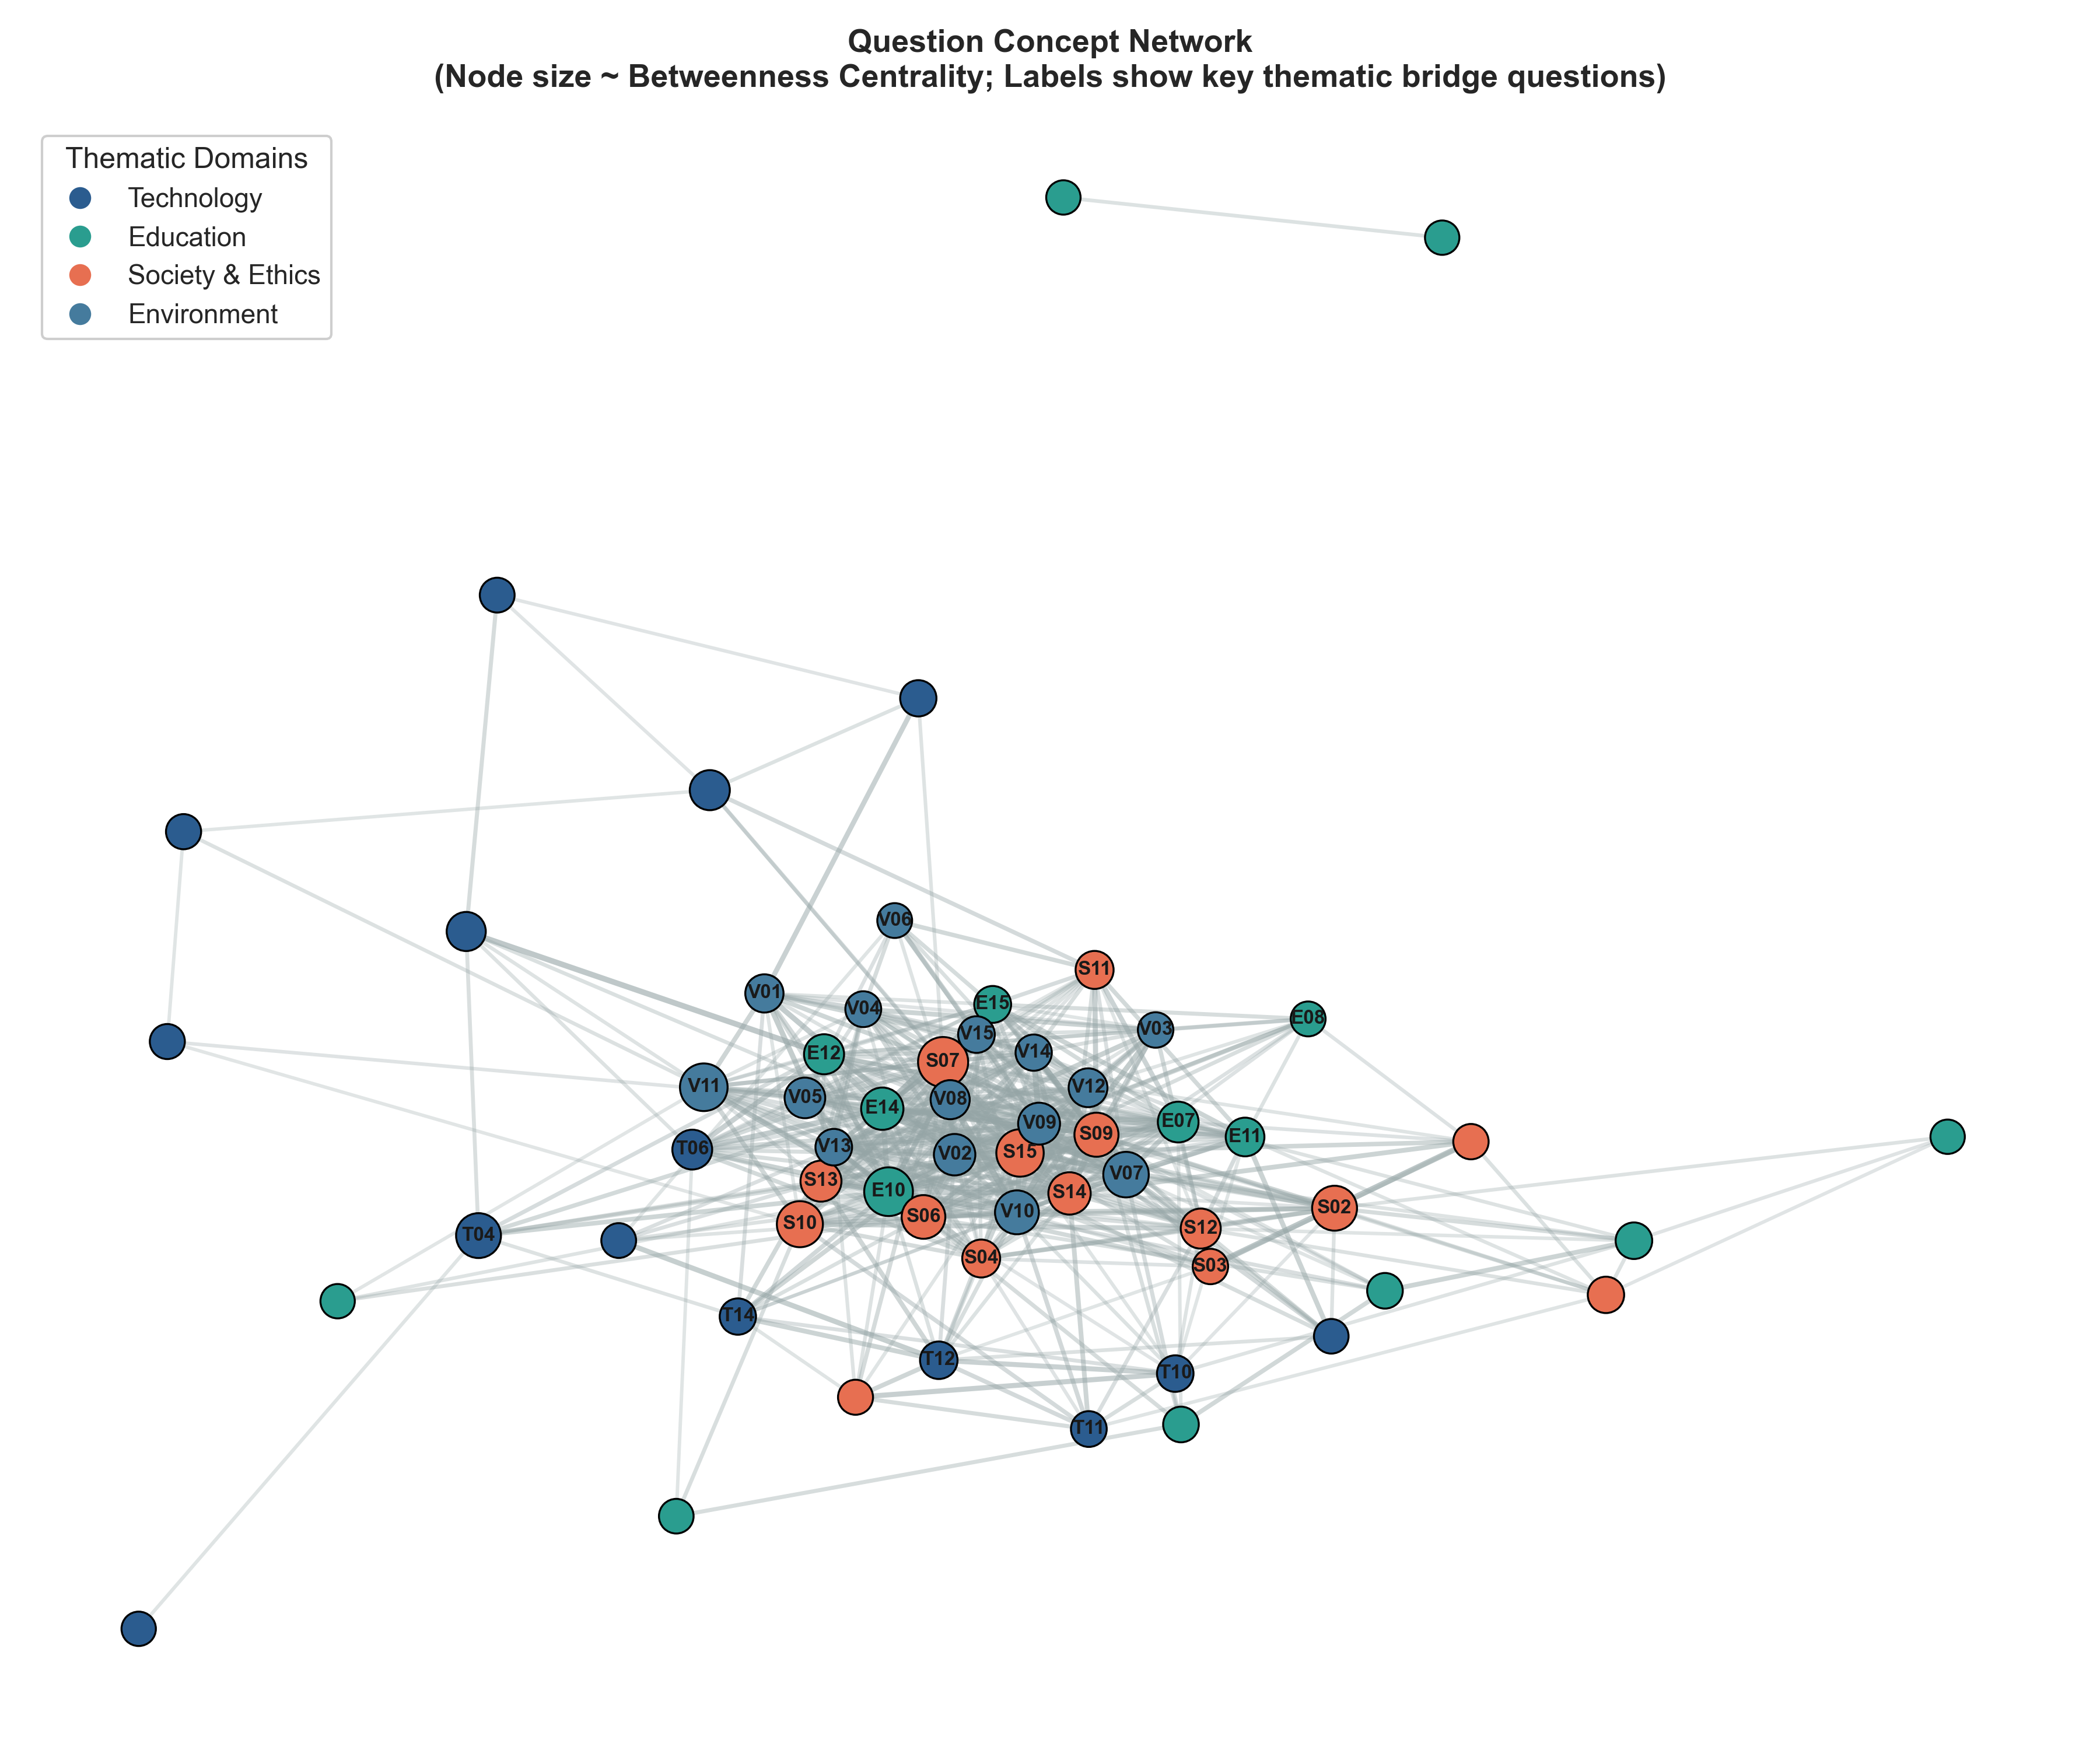
\includegraphics[width=\columnwidth]{figures/fig6_question_thematic_network.png}
\caption{Question Concept Network ($G_Q$ at $\tau^*_Q = 0.25$, $N=60, M=470$). Node colors denote domains; node sizes scale with Betweenness Centrality.}
\label{fig:question_network_vis}
\end{figure}

\subsection{Question Concept Network and Thematic Bridges}
Figure~\ref{fig:question_network_vis} visualizes $G_Q$ at $\tau^*_Q = 0.25$. The network forms a 58-node Giant Component alongside a disconnected 2-node component $\{\textbf{E02}, \textbf{E03}\}$, which correlate together ($r \ge 0.25$) but detach from the rest of the concept graph.

Top cross-thematic bridge questions by betweenness centrality:
\begin{enumerate}[noitemsep,topsep=1pt,leftmargin=1.2em]
    \item \textbf{S07 ($C_B = 0.0563$, Deg 29):} \textit{Equal opportunities regardless of background.}
    \item \textbf{E10 ($C_B = 0.0504$, Deg 31):} \textit{Innovation and problem-solving over rote learning.}
    \item \textbf{V11 ($C_B = 0.0460$, Deg 22):} \textit{Technology essential for environmental challenges.}
    \item \textbf{S15 ($C_B = 0.0450$, Deg 27):} \textit{Public trust for responsible emerging technologies.}
\end{enumerate}

These findings demonstrate that cross-domain connectivity is anchored by \textbf{equity ($S07$), pedagogical reform ($E10$), and the technology-environment nexus ($V11$)}.

\subsection{Methodological Limitations}
\begin{enumerate}[noitemsep,topsep=1pt,leftmargin=1.2em]
    \item \textbf{Static Response Topology:} Edges denote statistical alignment in survey response space rather than direct interpersonal communication, friendship, or social influence. While correlation networks accurately map ideological cohesion, they do not capture dynamic opinion propagation over time.
    \item \textbf{Degree-Unmatched Null Model:} The Erd\H{o}s--R\'enyi random baseline $G(N, p)$ assumes independent edge probabilities and a Poisson degree distribution, which does not preserve the empirical degree sequence. A degree-preserving configuration model or Chung--Lu model would provide an even more stringent benchmark for small-world validation.
    \item \textbf{Interval Assumption on Ordinal Data:} Pearson correlation assumes equal-interval distances between discrete Likert response levels. Although zero-centered scaling preserves symmetry, future studies could explore polychoric correlation or distance metric learning tailored to ordinal scales.
    \item \textbf{Sample Specificity and Generalizability:} The empirical dataset reflects a specific cohort of undergraduate engineering students ($N=87$). The observed high consensus on sustainability and data privacy may reflect domain-specific training rather than broader societal distributions.
\end{enumerate}

% ==============================================================================
% SECTION 7: INDIVIDUAL CONTRIBUTION
% ==============================================================================
\section{Individual Contribution}
\label{sec:contribution}

All team members contributed equitably ($33.3\%$ each) to the conceptualization, mathematical formulation, code implementation, figure generation, and report writing for this assignment. The individual task allocation and verified contribution breakdown are structured below:

\begin{description}[noitemsep,topsep=2pt,leftmargin=1.0em]
    \item[\textbf{Ampilli Sai Venkata Naga Bhargav}] (\textit{2023112014}): Erd\H{o}s--R\'enyi null model simulation ensemble ($N=50$), Small-World Index computation, zero-centered Likert scale mathematical encoding, Model 1 percolation threshold sweep implementation, and Louvain community detection algorithm formulation.
    \item[\textbf{Chaitanya Thogata}] (\textit{2023113018}): Model 1 network construction, Pearson similarity formulation, node centrality computations (Degree, Betweenness, Closeness), and consensus hub vs. topological bridge comparative analysis.
    \item[\textbf{Pasumarthy Deepak}] (\textit{2023101109}): missing-value imputation strategy (median), Survey data ingestion, Model 2 (Question Concept Network and percolation sweep), generation of publication figures, and comprehensive report compilation.
\end{description}

% ==============================================================================
% SECTION 8: CONCLUSION
% ==============================================================================
\section{Conclusion}
\label{sec:conclusion}

In this study, we transformed high-dimensional survey responses into dual complex networks to analyze opinion organization across Technology, Education, Society, and Environment. Through quality filtering ($N=87$) and percolation thresholding ($\tau^*_S = 0.35, \tau^*_Q = 0.25$), we established that the Student Opinion Network exhibits structural properties of \textbf{small-world organization ($\sigma = 1.8469$)}, combining elevated clustering ($\gamma = 1.9015$) with short geodesic paths ($\lambda = 1.0295$). Weighted Louvain community detection ($Q = 0.1293$) identified four primary ideological cohorts connected via a distributed core of consensus hubs and bridge students. Question-level analysis revealed that institutional educational policies constitute the primary axis of cohort polarization, while inter-domain conceptual connectivity is sustained by foundational principles of social equity, educational innovation, and sustainable technology.


\end{document}
